%convert -coalesce launch.gif launch_%d.png
\documentclass{beamer}

\newcommand{\VEV}[1]{\langle#1\rangle}
\newcommand{\sst}{\left(1-\frac{2M}{r}\right)}
\newcommand{\sh}{\mathrm{shell}}
\newcommand{\be}{\begin{equation}}
\newcommand{\ee}{\end{equation}}
\newcommand{\bue}{\begin{equation}}
\newcommand{\eue}{\end{equation}}
\newcommand{\bc}{\begin{center}}
\newcommand{\ec}{\end{center}}
\newcommand{\bea}[1]{\begin{eqnarray}\label{#1}}
\newcommand{\eea}{\end{eqnarray}}
\newcommand{\bua}{\begin{eqnarray*}}
\newcommand{\eua}{\end{eqnarray*}}
\newcommand{\dd}[2]{{{d#1}\over{d#2}}}
\newcommand{\ddt}[1]{\dd{#1}{t}}
\newcommand{\dddt}[1]{\dd{^2#1}{t^2}}
\newcommand{\aver}[1]{\langle{#1}\rangle}
\newcommand{\atom}[3]{\ifmmode^{#1}_{#2}{\rm{#3}}\else{$^{#1}_{#2}${#3}}\fi}
\newcommand{\electron}{\atom{~0}{-1}{e}}
\newcommand{\positron}{\atom{0}{0}{\bar{e}}}
\newcommand{\neutrino}{\atom{0}{0}{\nu_e}}
\newcommand{\photon}{\atom{0}{0}{\gamma}}
\newcommand{\antineutrino}{\atom{0}{0}{\bar{\nu}}}
\newcommand{\neutron}{\atom{1}{0}{n}}
\newcommand{\proton}{\atom{1}{1}{p}}
\newcommand{\hydrogen}{\atom{1}{1}{H}}
\newcommand{\deuterium}{\atom{2}{1}{H}}
\newcommand{\tritium}{\atom{3}{1}{H}}
\newcommand{\helium}{\atom{4}{2}{He}}
\newcommand{\hethree}{\atom{3}{2}{He}}

\renewcommand{\ss}{Schwarz\-schild }

\def\densu{kg/m$^3$} 
\def\rsol{R$_{\odot}$} 
\def\msol{M$_{\odot}$} 


\usetheme{Boadilla}
%\usepackage{multimedia}
%\usepackage{animate}
\usepackage{hyperref}
\usepackage{tikz}
\usepackage{cancel}
\usepackage{tikzsymbols}
\usepackage{ifthen}

%%%%mathcircled
\makeatletter
\newcommand\mathcircled[1]{%`
  \mathpalette\@mathcircled{#1}%
}
\newcommand\@mathcircled[2]{%
  \tikz[baseline=(math.base)] \node[draw,circle,red, thick, inner sep=2pt] (math) {$\m@th#1#2$};%
}
\makeatother
%%%%

%gets rid of bottom navigation bars
\setbeamertemplate{footline}[frame number]{}

%gets rid of bottom navigation symbols
\setbeamertemplate{navigation symbols}{}

%gets rid of footer
%will override 'frame number' instruction above
%comment out to revert to previous/default definitions
\setbeamertemplate{footline}{}

\definecolor{darkscarlet}{rgb}{0.34, 0.01, 0.1}
\definecolor{gold(metallic)}{rgb}{0.83, 0.69, 0.22}
\definecolor{green(ryb)}{rgb}{0.4, 0.69, 0.2}
\definecolor{darkorange}{rgb}{1.0, 0.55, 0.0}
\definecolor{amber}{rgb}{1.0, 0.75, 0.0}
\definecolor{bronze}{rgb}{0.8, 0.5, 0.2}
\definecolor{cadet}{rgb}{0.33, 0.41, 0.47}
\definecolor{silver}{rgb}{0.75, 0.75, 0.75}
\definecolor{turquoise}{rgb}{0.19, 0.84, 0.78}
\definecolor{uclagold}{rgb}{1.0, 0.7, 0.0}
\definecolor{urobilin}{rgb}{0.88, 0.68, 0.13}
\definecolor{vegasgold}{rgb}{0.77, 0.7, 0.35}
\definecolor{vanilla}{rgb}{0.95, 0.9, 0.67}
\definecolor{straw}{rgb}{0.89, 0.85, 0.44}
\definecolor{sunset}{rgb}{0.98, 0.84, 0.65}
\definecolor{brown(traditional)}{rgb}{0.59, 0.29, 0.0}
\definecolor{apricot}{rgb}{0.98, 0.81, 0.69}
\definecolor{darkblue}{rgb}{0,0,0.54}
\definecolor{aquamarine}{rgb}{0.5, 1.0, 0.83}

\hypersetup{
    colorlinks=true,
    linkcolor=yellow,
    filecolor=magenta,      
    urlcolor=blue,
}

\let\hrefori\href
\renewcommand{\href}[2]{{\setlength{\fboxsep}{1pt}\colorbox{sunset}{\hrefori{#1}{#2}}}}


%title
\setbeamercolor{block title alerted}{fg=white,bg=cyan}
%body
\setbeamercolor{block body alerted}{fg=black!90,bg=yellow!60}

%title
\setbeamercolor{block title}{fg=black,bg=turquoise}
%body
\setbeamercolor{block body}{fg=yellow,bg=bronze}



\newcommand\setItemnumber[1]{\setcounter{enumi}{\numexpr#1-1\relax}}

\newcommand{\pagebutton}[1]{\setbeamertemplate{button}{\tikz\node[inner xsep = 5pt, draw = structure!90, fill = green(ryb), rounded corners = 8pt]{\color{amber}\Large\insertbuttontext};}\beamerbutton{#1}}

\newcommand{\choicebutton}[1]{\setbeamertemplate{button}{\tikz\node[inner xsep = 8pt, draw = structure!90, fill = vegasgold, rounded corners = 5pt]{\color{vanilla}\Large\insertbuttontext};}\beamerbutton{#1}}

\newcommand{\pagenobutton}[1]{\setbeamertemplate{button}{\tikz\node[inner xsep = 8pt, draw = structure!90, fill = apricot, rounded corners = 5pt]{\color{brown(traditional)}\Large\insertbuttontext};}\beamerbutton{#1}}

\newcommand{\headlinebutton}[1]{\setbeamertemplate{button}{\tikz\node[inner xsep = 8pt, draw = structure!90, fill = blue, rounded corners = 5pt]{\color{yellow}\Large\insertbuttontext};}\beamerbutton{#1}}

\newcommand{\forumbutton}{\href{https://astro-discourse.utenforuio.no/c/ast2000/sporsmal-til-forelesningsnotater-del-1a-1g/16}{\setbeamertemplate{button}{\tikz\node[inner xsep = 8pt, draw = structure!90, fill = darkblue, rounded corners = 5pt]{\color{yellow}\Large\insertbuttontext};}\beamerbutton{\textcolor{red}{\small FORUM}}}}

\newcommand{\curpage}{\pagenobutton{\small side \thepageno\  av \thenopages}}
\newcommand{\nextpage}{\refstepcounter{pageno}\pagenobutton{\small side \thepageno\  av \thenopages}}
\newcommand{\dnextpage}{\refstepcounter{pageno}\refstepcounter{pageno}\pagenobutton{\small side \thepageno\  av \thenopages}}

\newcommand{\lastpagebutton}[1]{\hyperlink{#1}{\pagebutton{\small Forrige side}}\href{https://nettskjema.no/a/160191}{\Changey[1][yellow]{2} \Changey[1][yellow]{-2}}\nextpage\headlinebutton{\headline}\forumbutton\\}
\newcommand{\clastpagebutton}[1]{\hyperlink{#1}{\pagebutton{\small Forrige side}}\href{https://nettskjema.no/a/160191}{\Changey[1][yellow]{2} \Changey[1][yellow]{-2}}\curpage\headlinebutton{\headline}\forumbutton\\}
\newcommand{\dlastpagebutton}[1]{\hyperlink{#1}{\pagebutton{\small Forrige side}}\href{https://nettskjema.no/a/160191}{\Changey[1][yellow]{2} \Changey[1][yellow]{-2}}\dnextpage\headlinebutton{\headline}\forumbutton\\}

\newcommand{\lastpagebuttonx}[1]{\hyperlink{#1}{\pagebutton{\small Forrige side}}\href{https://nettskjema.no/a/160191}{\Changey[1][yellow]{2} \Changey[1][yellow]{-2}}\nextpage\\}
\newcommand{\clastpagebuttonx}[1]{\hyperlink{#1}{\pagebutton{\small Forrige side}}\href{https://nettskjema.no/a/160191}{\Changey[1][yellow]{2} \Changey[1][yellow]{-2}}\curpage\\}
\newcommand{\dlastpagebuttonx}[1]{\hyperlink{#1}{\pagebutton{\small Forrige side}}\href{https://nettskjema.no/a/160191}{\Changey[1][yellow]{2} \Changey[1][yellow]{-2}}\dnextpage\\}

\newcommand{\lastpagebuttoncr}[1]{\hyperlink{#1}{\pagebutton{\small Forrige side}}\href{https://nettskjema.no/a/160191}{\Changey[1][yellow]{2} \Changey[1][yellow]{-2}}\nextpage\\\headlinebutton{\headline}\forumbutton\\}
\newcommand{\clastpagebuttoncr}[1]{\hyperlink{#1}{\pagebutton{\small Forrige side}}\href{https://nettskjema.no/a/160191}{\Changey[1][yellow]{2} \Changey[1][yellow]{-2}}\curpage\\\headlinebutton{\headline}\forumbutton\\}
\newcommand{\dlastpagebuttoncr}[1]{\hyperlink{#1}{\pagebutton{\small Forrige side}}\href{https://nettskjema.no/a/160191}{\Changey[1][yellow]{2} \Changey[1][yellow]{-2}}\dnextpage\\\headlinebutton{\headline}\forumbutton\\}

\newcommand{\nytemaside}[1]{
\centerline{\Huge\textcolor{yellow}{Nytt tema:}}\\
\vspace*{1cm}
\centerline{\Large\bf\textcolor{yellow}{\headline}}
\vspace*{2cm}
\ifthenelse{\equal{#1}{0}}{\centerline{\textcolor{yellow}{Siste tema i denne forelesningen!}}}{\centerline{\textcolor{yellow}{\footnotesize Dette temaet fortsetter frem til side \ref{#1} av \thenopages.}}}
\vspace*{0.5cm}
}


\newcommand{\fullframe}[5]{
\begin{frame}
\label{#1}
\addtocounter{pageno}{#4}
\lastpagebutton{#2}
#5
\hyperlink{#3}{\pagebutton{Neste side}}
\end{frame}
}



\newcommand{\fullframetwo}[6]{
\begin{frame}
\label{#1}
\addtocounter{pageno}{#4}
\lastpagebutton{#2}
\begin{columns}
\column{0.5\textwidth}
#5
\column{0.5\textwidth}
#6
\hyperlink{#3}{\pagebutton{Neste side}}
\end{columns}
\end{frame}
}



\newcommand{\fullframetxt}[6]{
\begin{frame}
\label{#1}
\addtocounter{pageno}{#4}
\lastpagebutton{#2}
#6
\hyperlink{#3}{\pagebutton{#5}}
\end{frame}
}

\newcommand{\choiceframe}[4]{
\begin{frame}
\label{#1}
\addtocounter{pageno}{#3}
\lastpagebutton{#2}
#4
\end{frame}
}

\newcommand{\colfullframe}[6]{
{
\setbeamercolor{background canvas}{bg=#5}
\begin{frame}
\label{#1}
\addtocounter{pageno}{#4}
\lastpagebutton{#2}
#6
\hyperlink{#3}{\pagebutton{Neste side}}
\end{frame}
}
}

\newcommand{\colfullframetwo}[7]{
{
\setbeamercolor{background canvas}{bg=#5}
\begin{frame}
\label{#1}
\addtocounter{pageno}{#4}
\lastpagebutton{#2}
\begin{columns}
\column{0.5\textwidth}
#6
\column{0.5\textwidth}
#7
\hyperlink{#3}{\pagebutton{Neste side}}
\end{columns}
\end{frame}
}
}

\newcommand{\colfullframetxt}[7]{
{
\setbeamercolor{background canvas}{bg=#5}
\begin{frame}
\label{#1}
\addtocounter{pageno}{#4}
\lastpagebutton{#2}
#7
\hyperlink{#3}{\pagebutton{#6}}
\end{frame}
}
}

\newcommand{\colchoiceframe}[5]{
{
\setbeamercolor{background canvas}{bg=#4}
\begin{frame}
\label{#1}
\addtocounter{pageno}{#3}
\lastpagebutton{#2}
#5
\end{frame}
}
}


\newcommand{\pagequestion}[3]{
\hyperlink{#1}{\pagebutton{#2}}
\pause
%#3 normalt -1 for første spørsmål
\addtocounter{pageno}{#3}
\begin{itemize}[<+->]
\item[] \hypertarget<.>{#1}{}
\end{itemize}
\vspace{-0.5cm}
}

\newcommand{\samepagequestion}[4]{
\hyperlink{#1}{\pagebutton{#2}}\hyperlink{#1}{\pagebutton{#3}}
\pause
%#3 normalt -1 for første spørsmål
\addtocounter{pageno}{#4}
\begin{itemize}[<+->]
\item[] \hypertarget<.>{#1}{}
\end{itemize}
\vspace{-0.5cm}
}

\newcommand{\twopagequestion}[7]{
\hyperlink{#1}{\pagebutton{#3}}\hyperlink{#2}{\pagebutton{#4}}
\pause
%#3 normalt -1 for første spørsmål
\addtocounter{pageno}{#5}
\begin{itemize}[<+->]
\item[] \hypertarget<.>{#1}{}
\end{itemize}
\vspace{-0.5cm}
#7
\addtocounter{pageno}{#6}
\begin{itemize}[<+->]
\item[] \hypertarget<.>{#1}{}
\end{itemize}
\vspace{-0.5cm}
}

\newcounter{pageno}
\newcounter{nopages}
\setcounter{nopages}{42}

\newcommand{\headline}{\small Introduksjon}

\begin{document}


%%%%% front

\begin{frame}
\label{front2}
\center{\Large \textcolor{darkscarlet}{\bf AST2000 Del 1C\\Interaktive forelesningsnotater: forelesning 2 av 2}}\\
\begin{block}{\center{\bf VIKTIG}}
\textcolor{yellow}{Dette er et alternativ til forelesningen i emnet.} \textcolor{yellow}{Har du gått skikkelig gjennom disse interaktive forelesningsnotatene så trenger du ikke å lese \href{https://www.uio.no/studier/emner/matnat/astro/AST2000/h21/undervisningsmateriell/lecture_notes/part1c.pdf}{de fulle forelesningsnotatene} (med unntak av oppgavene bak)}. All informasjonen du trenger, får du her. Du kommer til å få mange grublespørsmål og diskusjonsoppgaver, det er meningen at disse skal gjøres i grupper av minst 2, maks 4 studenter. {\bf Det er defor sterkt anbefalt at dere sitter sammen i grupper når dere går gjennom disse interaktive forelesningsnotatene, du vil få betydelig mer utbytte av dem på den måten}. {\bf Hvis du har kommentarer ris/ros til disse forelesningsnotatene eller til emnet, trykk på \href{https://nettskjema.no/a/160191}{\Changey[1][yellow]{2} \Changey[1][yellow]{-2}}\ knappen som du finner på alle sider.}
\end{block}
%\setbeamercolor{button}{bg=black,fg=yellow}
\hyperlink{front3}{\pagebutton{Trykk denne knappen for å begynne}}
\end{frame}

\begin{frame}
\label{front3}
{\Large
\begin{itemize}
\item HUSK at du får mer ut av de interaktive forelesningsnotatene når du gjør de sammen med noen. Diskusjonene med andre er svært viktige.
\item Det er mange spørsmål/grubliser underveis, sett dere selv en tidsgrense, 1 minutt på de korte, maks 4-5 minutter på de lenger. Ha en alarm ved siden av, ellers kommer dere til å bruke alt for langt tid. Har dere ikke fått det til etter kort tid, gå videre, se svaret og lær!
\item Er du i det minste tvil om noe, så finnes det en \forumbutton knapp, trykk det og still spørsmål med en gang mens du enda husker spørsmålet!
\end{itemize}
}
\hyperlink{tableofcontents}{\pagebutton{Trykk denne knappen for å begynne}}
\end{frame}


\begin{frame}
\label{tableofcontents}
\hyperlink{front3}{\pagebutton{Forrige side}}\\
Hvis du allerede har begynt på denne forelesningen og vil hoppe rett inn til et annet kapittel, kan du trykke her:
\begin{itemize}
\item \hyperlink{blue_nytema1}{\headlinebutton{Et eksempel}}
\item \hyperlink{blue_nytema2}{\headlinebutton{Støy i data: Teoretisk modell}}
\item \hyperlink{blue_nytema3}{\headlinebutton{Minste kvadraters metode}}
\item \hyperlink{blue_nytema4}{\headlinebutton{Støy i data:statistikk}}
\item \hyperlink{blue_nytema5}{\headlinebutton{Tips til parameterestimering}}
\end{itemize}
\hyperlink{intro}{\choicebutton{Neste side}}
\end{frame}

%%%%% intro
\begin{frame}
\label{intro}
\begin{columns}
\column{0.5\textwidth}
\hyperlink{tableofcontents}{\pagebutton{Forrige side}}\\
\vspace{1cm}
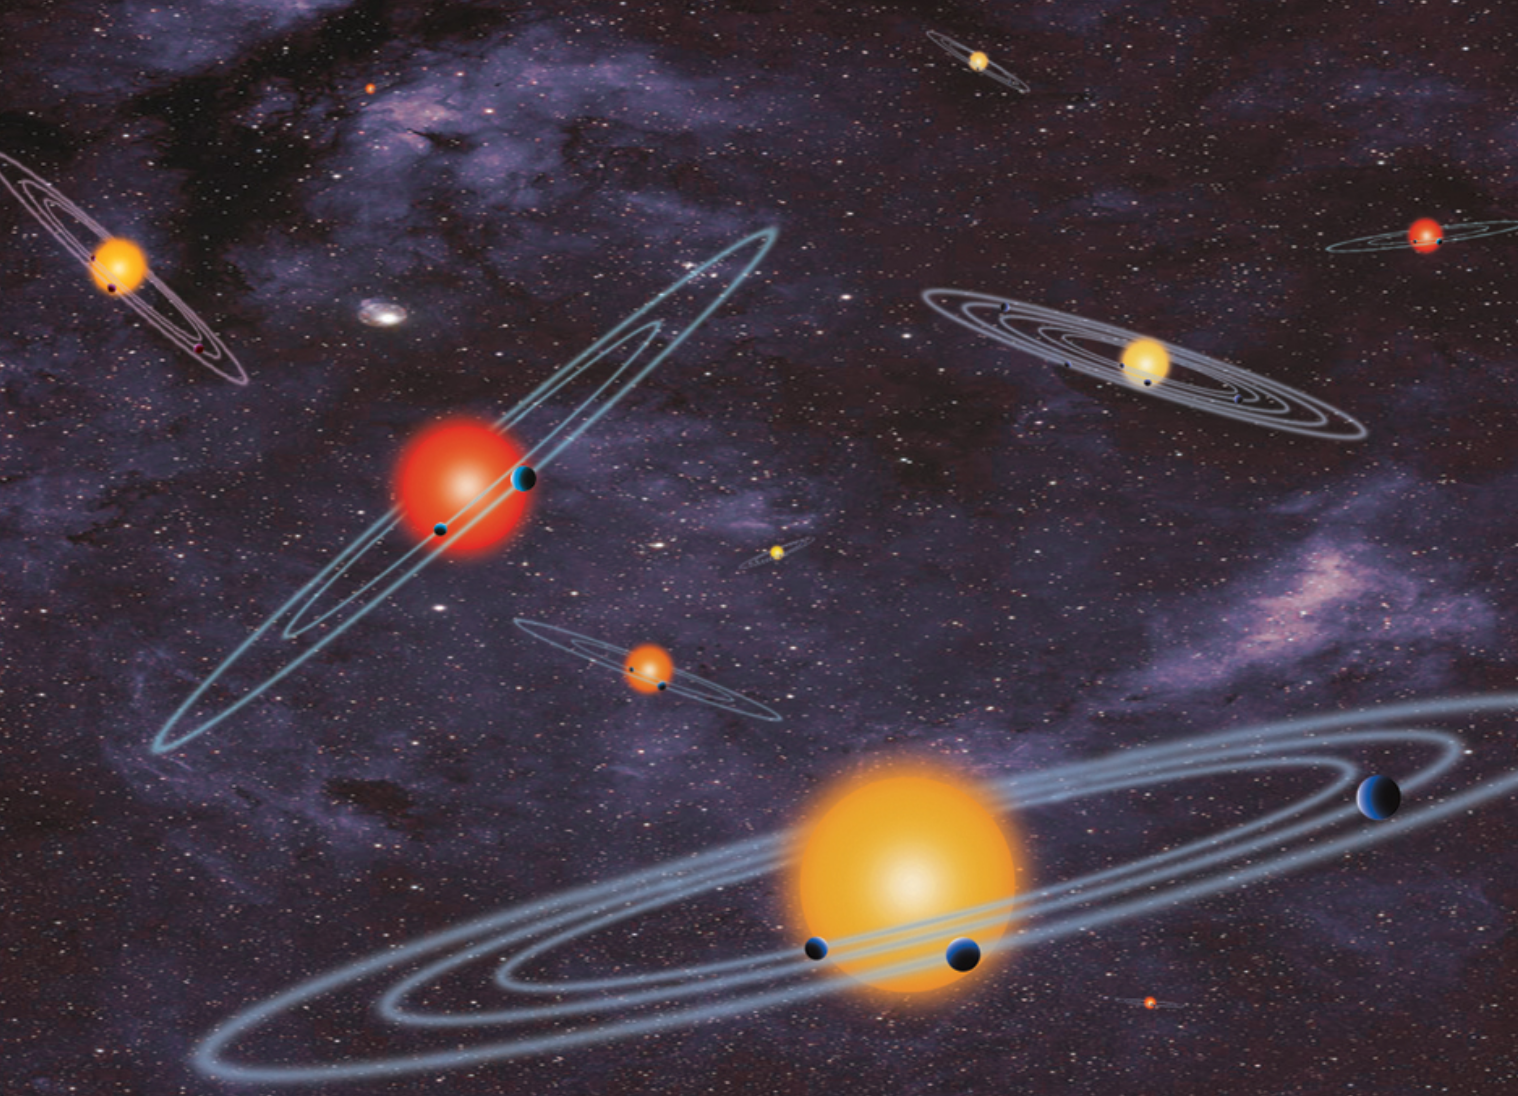
\includegraphics[scale=0.22]{media/extrasolarplanets.png}\\
\column{0.5\textwidth}
\small Velkommen til andre forelesning av del 1C! Vi skal begynne med å bruke det du lærte i første forelesning på noen eksempler. Deretter skal vi se hvordan vi kan analysere data med støy, og du skal lære å estimere planetmasser fra mer realistiske stjernedata. Dette forelesningsnotatet tilsvarer omtrent en dobbelttime fysisk forelesning. \\{\bf Er du klar?}\\\vspace*{1cm}\hyperlink{intro2}{\pagebutton{Neste side}}
%\movie[autostart]{testmovie}{launch.gif}%bate2.mpg
\end{columns}
\end{frame}

\begin{frame}
\label{intro2}
\lastpagebutton{intro}
{\small
Vi utledet i forrige forelesning sammenhengen mellom stjernas banehastighet og massen til planeten som går i bane rundt stjerna
\[
m_p=\left(\frac{P}{2\pi G}\right)^{1/3}m_*^{2/3}\frac{v_{*r}}{\sin{i}}
\]
der $P$ er omløpsperioden, $i$ er inklinasjonen ({\bf husker du hvordan den er definert? Hvis ikke, gå tilbake og sjekk nå!)}, stjernas masse $m_*$ som vi kan regne som kjent og til slutt $v_{*r}$ som er stjernas observerte radielle komponent av banehastighet i banen om massesenteret. Dopplereffekten gjør at vi kan finne stjernas radialhastighet {\bf (sjekk at du husker definisjon av radialhastighet og tangensialhastighet fra observatøren)} på forskjellige tidspunkter ved å se på bølgelegnden til en spektrallinje. Fra hastighetskurven til stjerna (radialhastiheten $v_r(t)$ som funksjon av tiden) kan vi finne banehastigheten $v_*$ til stjerna {\bf(sjekk at du husker hvordan du leser den av fra kurven)}.\\
\textcolor{blue}{Inklinasjonen $i$ er vanskelig å finne, men ved $i=90^\circ$ kan vi få en formørkelse av stjerna hver gang planeten går foran. Deg gjør at vi kan måle radiusen til planeten hvis vi har gode data ved at $2R_p=v_p(t_1-t_0)$. {\bf Husker du hvilke tidspunkter $t_0$ ot $t_1$ du må lese av og hvorfor disse tidspunktene? Du bør kunne utlede denne sammenhengen!}}
\hyperlink{blue_nytema1}{\pagebutton{Neste side}}
}
\end{frame}

\renewcommand{\headline}{\small Et eksempel}
{
\setbeamercolor{background canvas}{bg=blue}
\begin{frame}
\label{blue_nytema1}
\hyperlink{intro2}{\pagebutton{\small Forrige side}}
\nytemaside{stoy}
\hyperlink{eks1}{\pagebutton{Sett igang med eksemplet!}}
\end{frame}
}

\begin{frame}
\label{eks1}
\lastpagebutton{intro2}
Vi skal gjøre deler av oppgave 1C.3 her. Vi skal se på en realistisk hastighetskurve med støy. Vi skal snart lære mer om støy, men den gir et tilfeldig ekstra utslag på hastighetskurven i hvert tidssted. {\bf Støyen gir et tilfeldig hastighetsbidrag i hvert tidssteg som i middel skal gå like mye opp som ned slik at den underliggende kurven uten støy ligger midt inne i støyen.}\\
\vspace*{0.5cm}
\begin{columns}
\column{0.5\textwidth}
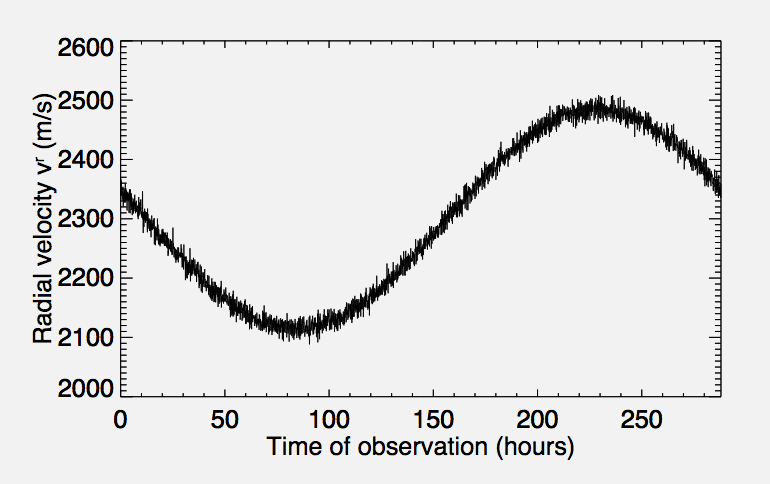
\includegraphics[scale=0.45]{media/1c3_1.png}\\
Her ser vi radialhastighetskurven til en stjerne.
\column{0.5\textwidth}
Anslå egenhastigheten til stjerna {\bf hvis du ikke husker hva egenhastighet var, gå tilbake til forrige forelesning, dette er et svært viktig konsept!}. Er den:\\
\hyperlink{feilv}{\choicebutton{0m/s}}\ \hyperlink{feilv}{\choicebutton{2500m/s}}\ \hyperlink{feilv}{\choicebutton{2475m/s}}\ \hyperlink{riktigv}{\choicebutton{2300m/s}}\ \hyperlink{feilv}{\choicebutton{2125m/s}}\ \hyperlink{feilv}{\choicebutton{2100m/s}}\ \hyperlink{feilv}{\choicebutton{400m/s}}\ \hyperlink{feilv}{\choicebutton{175m/s}}\ 
\end{columns}
\end{frame}

{
\setbeamercolor{background canvas}{bg=black}
\begin{frame}
\label{feilv}
\lastpagebutton{eks1}
\textcolor{white}{Det ble galt. Er du sikker på at du forstår hva egenhastighet er for noe? Egenhastigheten er hastigheten til massesenteret. Stjerna har hastigheten til massesenteret pluss banehastighet omkring massesenteret. Gå tilbake til forrige forelesning og kontroller at du forstår godt hvorfor hastighetskurven ser ut slik som den ser ut. Hvis du ikke forstår dette må du ikke gå videre da vil du ikke få noe ut av denne forelesningen. Tenk og gjør et nytt forsøk. Hvis du etter det enda ikke forstår, kikk på \href{https://www.uio.no/studier/emner/matnat/astro/AST2000/h20/undervisningsressurser/interaktive-forelesningsnotater/1c/videoer/video1c_6.mp4}{denne videoen}.}
\end{frame}
}

{
\setbeamercolor{background canvas}{bg=yellow}
\begin{frame}
\label{riktigv}
\clastpagebutton{eks1}
Bra! Du ser ut til å ha forstått hastighetskurven og at egenhastigheten er massesenterets hastighet. Hvis du likevel skulle være litt i tvil, så kikk gjerne på \href{https://www.uio.no/studier/emner/matnat/astro/AST2000/h20/undervisningsressurser/interaktive-forelesningsnotater/1c/videoer/video1c_6.mp4}{denne videoen} som forklarer det i litt detalj.
\hyperlink{eks2}{\pagebutton{Neste side}}
\end{frame}
}



\begin{frame}
\label{eks2}
\lastpagebutton{eks1}
Vi fortsetter med deler av oppgave 1C.3 her:\\
\vspace*{1cm}
\begin{columns}
\column{0.5\textwidth}
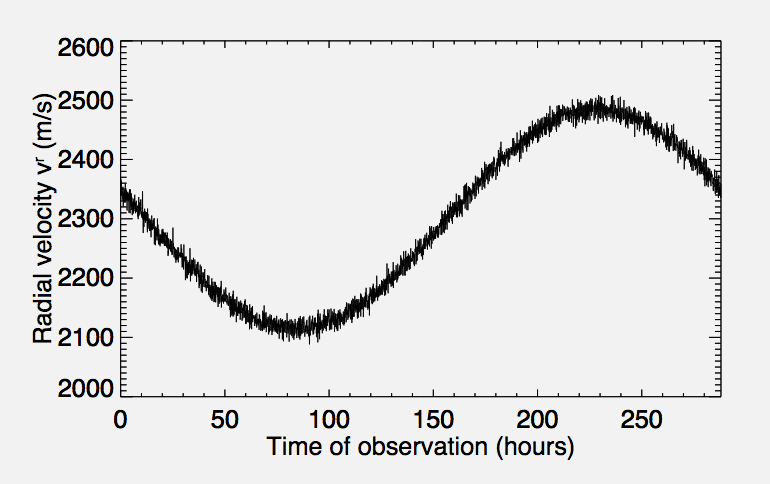
\includegraphics[scale=0.45]{media/1c3_1.png}\\
Her ser vi radialhastighetskurven til en stjerne.
\column{0.5\textwidth}
Hvis vi antar at inklinasjonen er $90^\circ$, anslå den fulle banehastigheten til stjerna i bane om massesenteret. Er den:\\
\hyperlink{feilv2}{\choicebutton{0m/s}}\ \hyperlink{feilv2}{\choicebutton{2500m/s}}\ \hyperlink{feilv2}{\choicebutton{2475m/s}}\ \hyperlink{feilv2}{\choicebutton{2300m/s}}\ \hyperlink{feilv2}{\choicebutton{2125m/s}}\ \hyperlink{feilv2}{\choicebutton{2100m/s}}\ \hyperlink{feilv2}{\choicebutton{400m/s}}\ \hyperlink{riktigv2}{\choicebutton{175m/s}}\ 
\end{columns}
\end{frame}


{
\setbeamercolor{background canvas}{bg=black}
\begin{frame}
\label{feilv2}
\lastpagebutton{eks2}
\textcolor{white}{Det ble ikke helt riktig. Kan det være at du har glemt at støyen gir like mye utslag opp som ned og at den virkelige hastighetskurven som vi er ute etter ligger midt inne i den støyete kurven? Eller kan det være at du har glemt at banehastigheten er hastigheten {\bf i forhold til massesenteret}? Tenk litt til, og prøv igjen!}
\end{frame}
}

{
\setbeamercolor{background canvas}{bg=yellow}
\begin{frame}
\label{riktigv2}
\clastpagebutton{eks2}
\begin{columns}
\column{0.5\textwidth}
Det er helt riktig! Siden banehastigheten er hastigheten {\bf i forhold til massesenteret}, så må vi se på det maksimale utslaget fra massesenterhastigheten. 
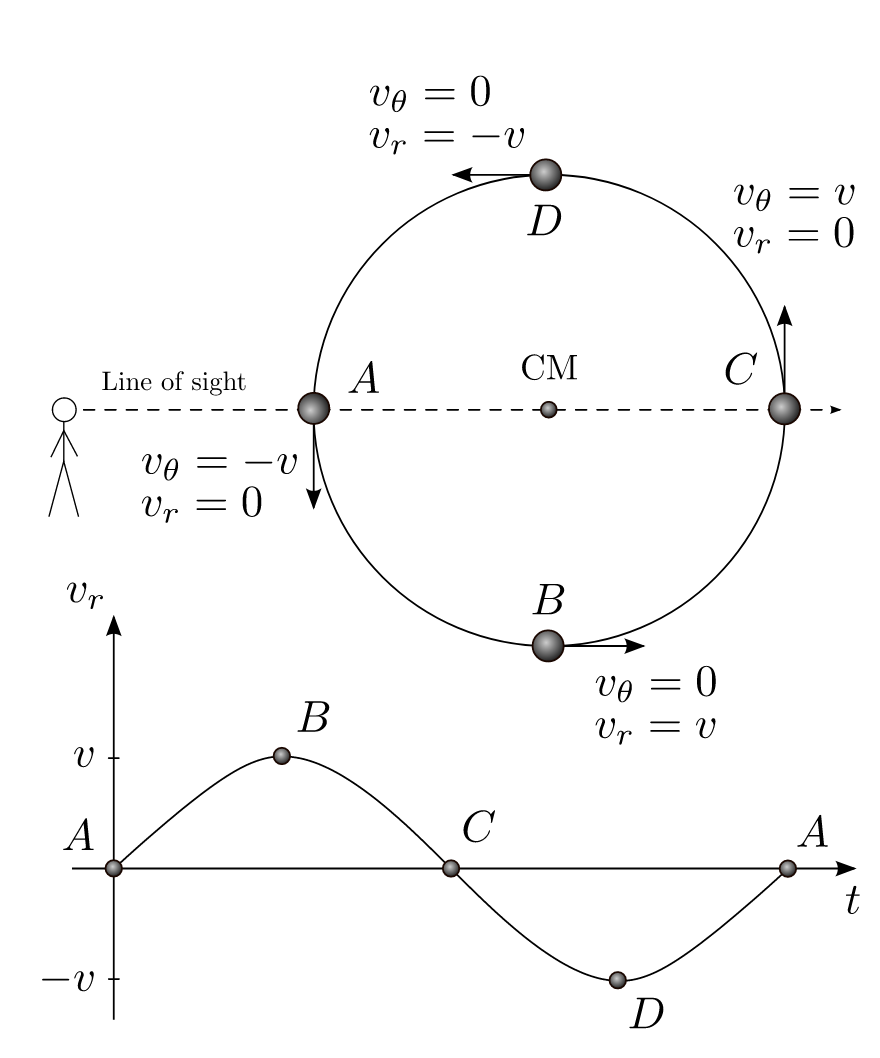
\includegraphics[scale=0.32]{media/vr.png}\\
\column{0.5\textwidth}
\parbox{\linewidth}{\textcolor{red}{Vi ser på det maksimale utslaget siden $v_r$-komponenten har den fulle hastigheten i punkt B på figuren (se forrige forelesning)}. Massesenter\-hastigheten er 2300m/s og det maksimale utslaget på toppen av kurven er ca. 2475m/s. {\bf MERK at det ikke er 2500 m/s siden dette er det maksimale utslaget {\bf med} støy.} Hvis den virkelige glatte kurven ligger midt inne i støyen slik at det er like mye støyutslag opp som ned, så må den vel ligge på ca. 2475m/s? Dermed har vi at 2475m/s-2300m/s = 175m/s (vi trekker altså fra massesenter\-hastigheten for å få hastighet i forhold til massesenteret).}
\hyperlink{eks3}{\pagebutton{Neste side}}
\end{columns}
\end{frame}
}


\begin{frame}
\label{eks3}
\lastpagebutton{riktigv2}
Hvis vi nå antar at inklinasjonen er ukjent, gjør et estimat av den minste mulige massen som denne planeten må ha. Anta at man ved spektroskopi har anslått stjernas masse til å være $0.3\mathrm{m}_\odot$ (merk at vi bruker $\mathrm{m}_\odot$ til å markere solmasser), altså en liten rød dvergstjerne. {\bf Her trenger du formelen fra forelesning 1 som er repetert i starten her av forelesning 2}
\begin{columns}
\column{0.5\textwidth}
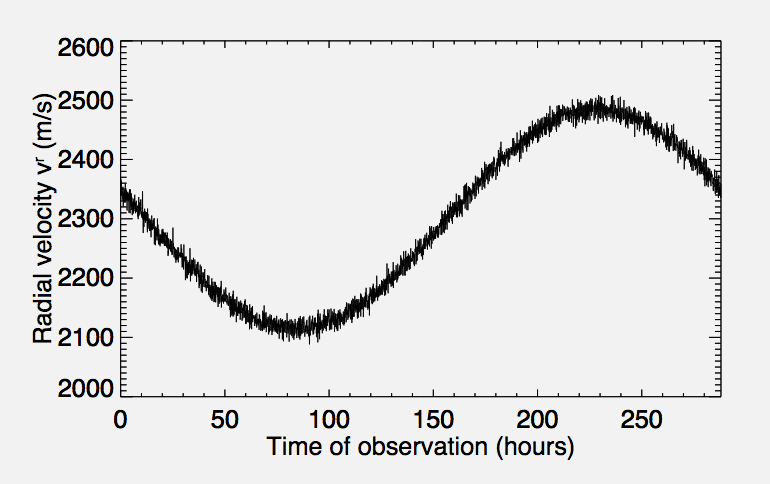
\includegraphics[scale=0.45]{media/1c3_1.png}\\
\column{0.5\textwidth}
Er den minste mulige massen:
\hyperlink{feilp}{\choicebutton{ca. 0.5 Jupitermasser}}\ \hyperlink{riktigp}{\choicebutton{ca. 0.9 Jupitermasser}}\ \hyperlink{feilp}{\choicebutton{ca. 1.3 Jupitermasser}}\ \hyperlink{feilp}{\choicebutton{ca. 2.1 Jupitermasser}}\ \hyperlink{feilp}{\choicebutton{ca. 2.8 Jupitermasser}}\ \hyperlink{feilp}{\choicebutton{ca. 3.5 Jupitermasser}}\ \hyperlink{feilp}{\choicebutton{ca. 4.9 Jupitermasser}}
\end{columns}
\end{frame}


{
\setbeamercolor{background canvas}{bg=black}
\begin{frame}
\label{feilp}
\lastpagebutton{eks3}
\textcolor{white}{Det ble nok ikke helt riktig. Usikkerheter i avlesninger gir litt slingringsmonn, men dette var litt for langt unna! Har du brukt $P=300$ timer, $v_*=175$m/s og $m_*=0.3m_\odot$? Hva får du hvis du bruker disse tallene? Blir det veldig forskjellig fra ditt tall? Gjør et nytt forsøk og spør gruppelærer hvis du ikke får det til.}
\end{frame}
}

{
\setbeamercolor{background canvas}{bg=yellow}
\begin{frame}
\label{riktigp}
\clastpagebutton{eks3}
Flott, du fikk det til! Kanskje du ikke fikk helt dette tallet? Det kan komme an på unøyaktigheter i avlesningen. Med $P=300$ timer, $v_*=175$m/s og $m_*=0.3m_\odot$ skulle du få et tall i nærheten av 0.9 jupitermasser.
\hyperlink{eks4}{\pagebutton{Neste side}}
\end{frame}
}


\begin{frame}
\label{eks4}
\lastpagebutton{riktigp}
Som du ser blir det ganske høy usikkerhet da det er vanskelig å lese av $P$ og $v_*$ nøyaktig med støy på kurven. Dette skal vi se nærmere på om et par sider. Men først skal vi jobbe litt mer med oppgave 1C.3. Vi fortsetter med den samme stjerna, men observasjoner av lyskurven viser at planeten formørker stjerna. Her ser vi utdrag av lyskurven fra en formørkelse:
\begin{columns}
\column{0.5\textwidth}
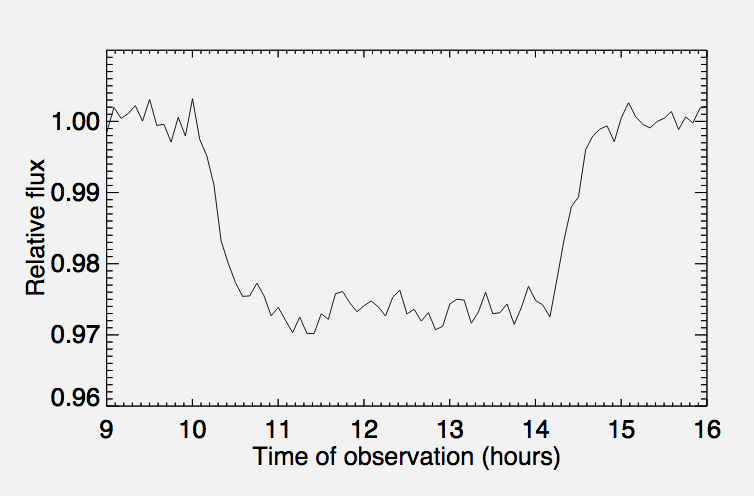
\includegraphics[scale=0.45]{media/1c3_2.png}\\
Gi et anslag på radiusen og tettheten til planeten. Du trenger kanskje å repetere fra forrige forelesning hvordan du finner $v_p$ (i forhold til CM) når du har $v_*$.
\column{0.5\textwidth}
Her blir det stor usikkerhet avhengig av hvordan du leser av den støyete kurven, svaret ditt ligger ikke nødvendigvis rett på et av disse, velg det nærmeste:\\
\vspace*{0.3cm}
\hyperlink{feilp2}{\choicebutton{\small ca. 0.5 Jupiterradier}}\ \hyperlink{feilp2}{\choicebutton{\small ca. 0.9 Jupiterradier}}\ \hyperlink{riktigp2}{\choicebutton{\small ca. 1.3 Jupiterradier}}\ \hyperlink{feilp2}{\choicebutton{\small ca. 2.1 Jupiterradier}}\ \hyperlink{feilp2}{\choicebutton{\small ca. 2.8 Jupitradier}}\ \hyperlink{feilp2}{\choicebutton{\small ca. 3.5 Jupiterradier}}
\end{columns}
\end{frame}

{
\setbeamercolor{background canvas}{bg=black}
\begin{frame}
\label{feilp2}
\lastpagebutton{eks4}
\textcolor{white}{Det ble nok ikke helt riktig. Usikkerheter i avlesninger gir litt slingringsmonn, men dette var litt for langt unna! Har du brukt at tiden fra planeten begynner å formørke stjernen til planeten formørker stjernen fullstendig er ca. 0.8 timer? Og at planethastigheten $v_p\approx 60$km/s? Hva får du hvis du bruker disse tallene? Blir det veldig forskjellig fra ditt tall? Gjør et nytt forsøk og spør gruppelærer hvis du ikke får det til.}
\end{frame}
}

{
\setbeamercolor{background canvas}{bg=yellow}
\begin{frame}
\label{riktigp2}
\clastpagebutton{eks4}
Flott, du fikk det til! Kanskje du ikke fikk helt dette tallet? Det kan komme an på unøyaktigheter i avlesningen. Med $v_p\approx 60$km/s og $t_1-t_0\approx0.8$ timer skulle du få et tall i nærheten av 1.3 jupiterradier. Vi ser altså at vi har en planet som er litt mindre massiv en jupiter men med noe større radius. Da får vi ca. 0.6 ganger tettheten til vann, litt mindre enn Saturn som har 0.7 ganger vannets tetthet. Dette er altså helt klart en gassplanet.
\[
\rho = \frac{0.9\times1.9\times10^{27}\mathrm{kg}}{\frac{4}{3}\pi(1.3\times70\times10^6\mathrm{m})^3}
\]
\hyperlink{eks5}{\pagebutton{Neste side}}
\end{frame}
}





\begin{frame}
\label{eks5}
\lastpagebutton{riktigp2}
{\bf Forstår du alle stegene? Hvis ikke, ta kontakt med foreleser eller gruppelærer!}\\
Husk at når vi karaktersetter prosjektet eller eksamen så er det forklaring av metoden som vi ser etter, ikke svaret. Når det gjelder estimering av planetmasser/radier, så er det fort gjort å venne seg til hvor man skal lese av på kurven og så sette disse tallene inn i en formel. Men da er det fort gjort å glemme {\bf hvorfor} man skal lese av på den måten og hvorfor formelen ser ut som den gjør. Det er \textcolor{red}{disse tingene} du blir testes i, {\bf ikke} om du kan lese av fra en kurve og sette inn i en formel, det forutsetter vi at du kan.\\
\vspace*{0.5cm}
Da har tiden kommet til å teste forståelsen din litt mer i \href{https://nettskjema.no/a/155695}{dette skjemaet}. Det kan ta litt tid å gå gjennom, men {\bf ikke} gå videre før du har sendt det inn da du trenger denne treningen i stoffet før du kan gå videre på statistikk og dataanalyse. {\bf Hvis du sliter med noen av spørsmålene i skjemaet, så er det svært viktig at du spør foreleser eller gruppelærer da skjemaet tester sentral forståelse som du kommer til å trenge videre i kurset.}
\hyperlink{blue_nytema2}{\pagebutton{Jeg har sendt inn skjemaet og er klar for dataanalyse-delen}}
\end{frame}

\renewcommand{\headline}{\small Støy i data: Teoretisk modell}

{
\setbeamercolor{background canvas}{bg=blue}
\begin{frame}
\label{blue_nytema2}
\hyperlink{eks5}{\pagebutton{\small Forrige side}}
\nytemaside{minstekvad}
\hyperlink{stat1}{\pagebutton{Strekk litt på bena først og trykk her!}}
\end{frame}
}

\begin{frame}
\label{stat1}
\lastpagebutton{eks5}\label{stoy}
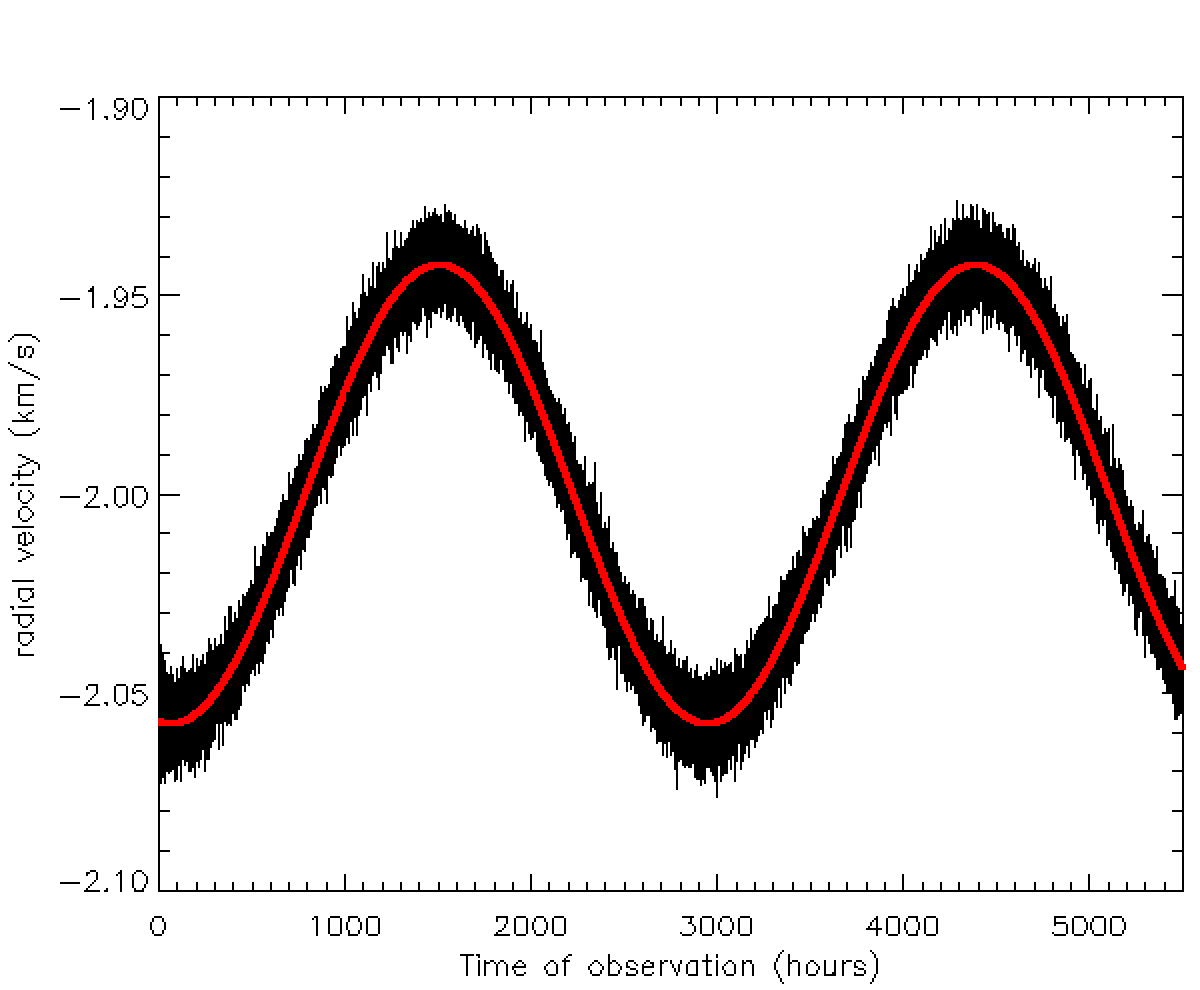
\includegraphics[scale=0.35]{media/vr_noisy.png}\\
{\small
I figuren ser vi en radialhastighetskurve tatt fra en spektrallinje i spektret fra en stjerne. Den røde linjen viser hvordan kurven hadde sett ut hvis det ikke var støy i måleinstrumentene. Den sorte kurven viser hva som faktisk måles og som gjør det vanskelig å trekke nøyaktige hastigheter ut av kurven.
}
\hyperlink{stat2}{\pagebutton{Neste side}}
\end{frame}



\begin{frame}
\label{stat2}
\begin{columns}
\column{0.5\textwidth}
\lastpagebuttonx{stat1}
\headlinebutton{\headline}
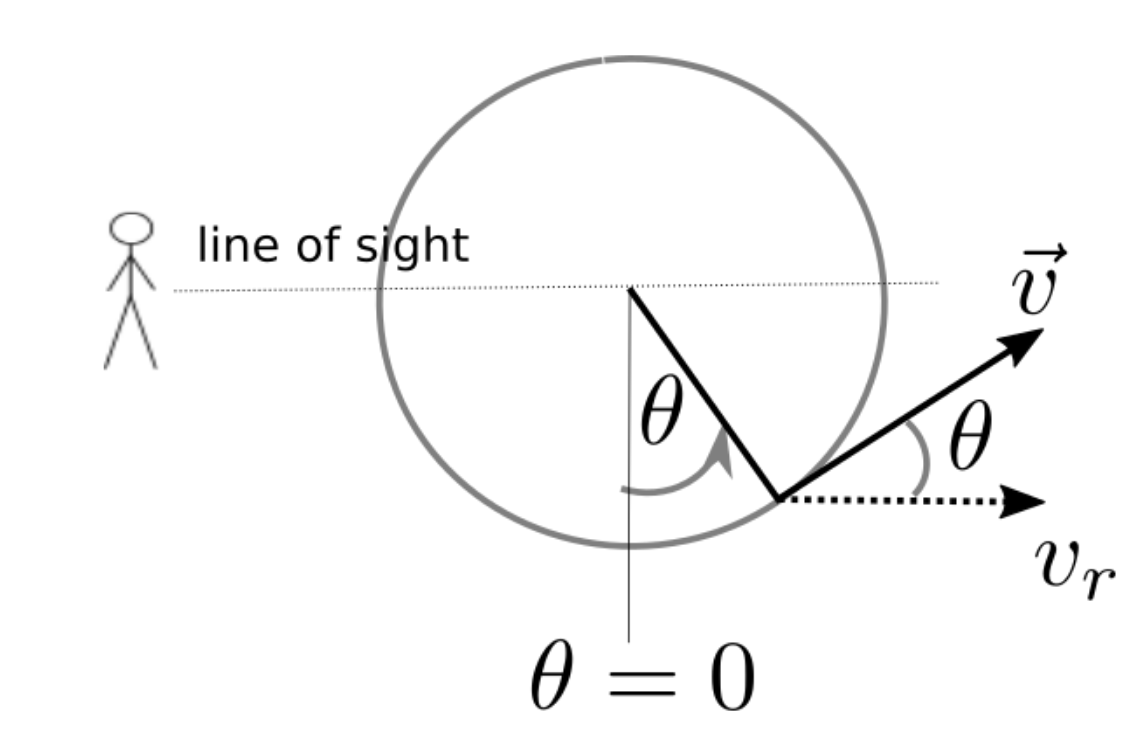
\includegraphics[scale=0.3]{media/vrmod.png}\\
{\small
Figuren viser stjerna i banen om massesenter med en vinkel $\theta$ som sier hvor i banen stjerna er. På figuren ser vi at $\theta$ også er vinkelen mellom $\vec{v}$ og synslinja.  Ser du hvorfor det er samme vinkel $\theta$ begge steder? ({\bf hint: en forlengelse av linja fra sentrum av sirkelen og radielt utover ved $\theta$).}.  
}
\column{0.5\textwidth}
{\small
For å kunne bruke kurven med støy til å finne mest mulig nøyaktige tall, trenger vi å lage en modell for den glatte 'virkelige' kurven som vi hadde observert hvis vi ikke hadde hatt støy. \textcolor{red}{Bruk figuren til å se om du kan utlede en analytisk modell for observert radialhastighet som funksjon av vinkelen $\theta(t)$ som er vist på figuren, samt den faktiske banehastigheten $v_*$ til banen (som er den vi er interessert i).}
}
\hyperlink{feilm}{\choicebutton{ $v_r(t)=v_*\sin{\frac{2\pi}{\theta(t)}}$}}\ \hyperlink{feilm}{\choicebutton{ $v_r(t)=v_*\cos{\frac{2\pi}{\theta(t)}}$}}\ \hyperlink{feilm}{\choicebutton{ $v_r(t)=v_*\sin{\theta(t)}$}}\ \hyperlink{riktigm}{\choicebutton{ $v_r(t)=v_*\cos{\theta(t)}$}}\ \hyperlink{feilm}{\choicebutton{ $v_r(t)=v_*\cos{\theta(t)}\sin{\theta}$}}\ \hyperlink{feilm}{\choicebutton{ $v_r(t)=v_*\tan{\theta(t)}$}}
\end{columns}
\end{frame}


{
\setbeamercolor{background canvas}{bg=black}
\begin{frame}
\label{feilm}
\lastpagebutton{stat2}
\textcolor{white}{Det ble feil, kansje du ikke kikket nøye nok på figuren? Innser du hvorfor $\theta$ som er vinkelen mellom $\vec{v}$ og $v_r$ må være samme vinkel som den $\theta$ som angir hvor på sirkelen stjernen er? Hvis du gjør det så ser du at $\theta$ er vinkelen mellom $\vec{v}$ og $v_r$ som betyr, som du jo vet, at $v_r$ er x-komponenten av $\vec{v}$? Dermed er $v_r$ projeksjonen av $\vec{v}$ med vinkelen $\theta$. Hjalp det? Gå tilbake og prøv igjen.}\\
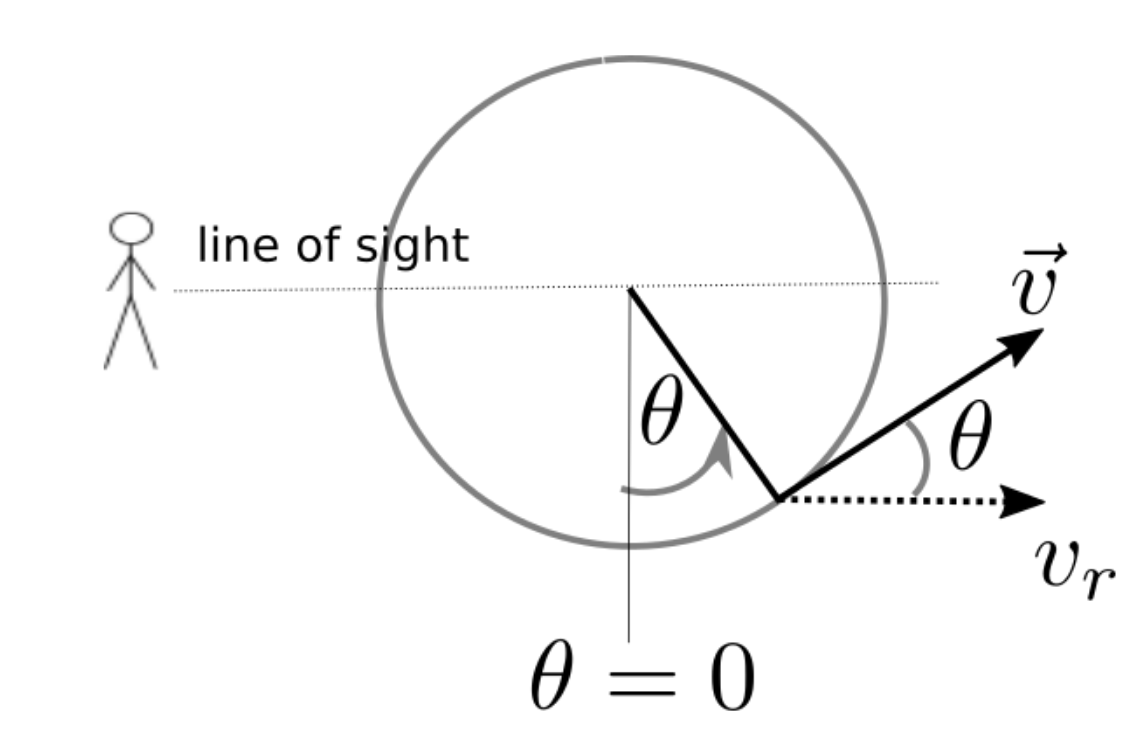
\includegraphics[scale=0.3]{media/vrmod.png}
\end{frame}
}

{
\setbeamercolor{background canvas}{bg=yellow}
\begin{frame}
\label{riktigm}
\clastpagebutton{stat2}
Helt riktig.  Innser du hvorfor $\theta$ som er vinkelen mellom $\vec{v}$ og $v_r$ må være samme vinkel som den $\theta$ som angir hvor på sirkelen stjernen er? Hvis du gjør det, så har du innsett at $v_r$ er x-komponenten til $\vec{v}$ med vinkel $\theta$ imellom og dermed er altså
\[
v_r(t)=v_*\cos{\theta(t)}
\]
\hyperlink{stat3}{\pagebutton{Neste side}}
\end{frame}
}



\begin{frame}
\label{stat3}
\lastpagebutton{riktigm}
\begin{columns}
\column{0.5\textwidth}
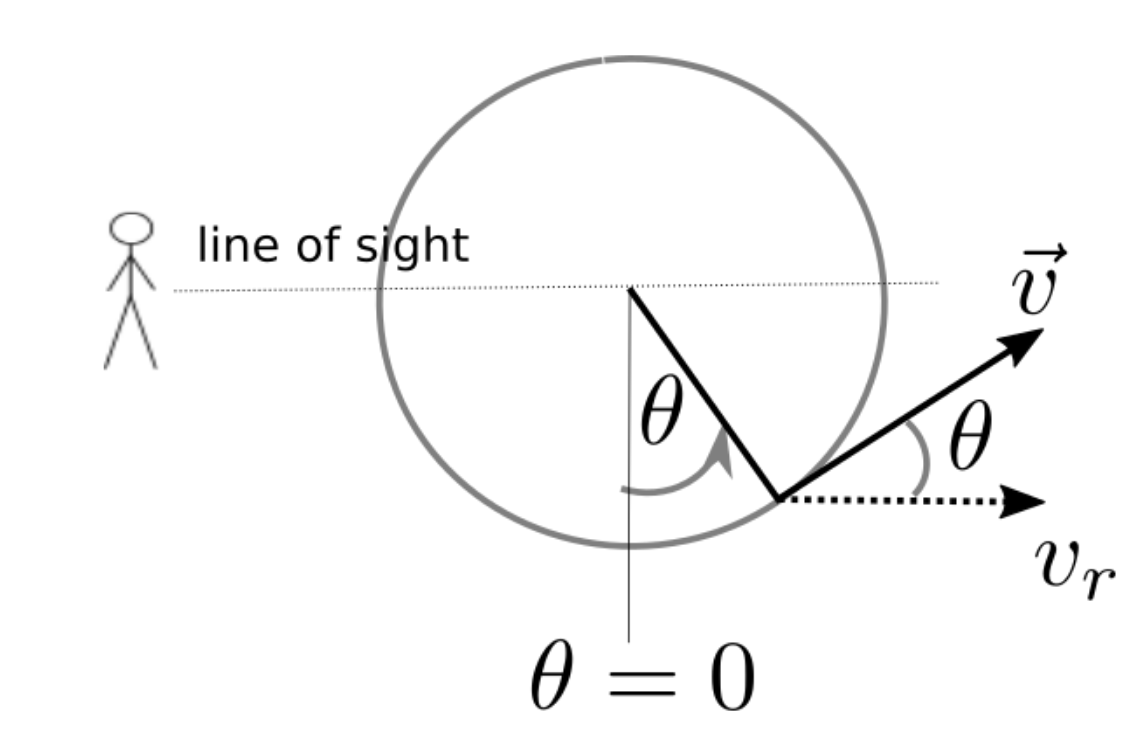
\includegraphics[scale=0.3]{media/vrmod.png}\\
Vi ble enige om at 
\[
v_r(t)=v_*\cos{\theta(t)}
\]
\column{0.5\textwidth}
Men for å ha en komplett modell, trenger vi også tidsavhengigheten til $\theta(t)$. Vi skal uttrykke den med omløpsperioden $P$. Anta at ved $t=0$ så er $\theta=0$ Er $\theta(t)$ lik:\\
\hyperlink{feilm2}{\choicebutton{ $\theta(t)=2\pi Pt$}}\ \hyperlink{feilm2}{\choicebutton{ $\theta(t)=\frac{P}{t}$}}\ \hyperlink{feilm2}{\choicebutton{ $\theta(t)=P\cos{2\pi t}$}}\ \hyperlink{feilm2}{\choicebutton{ $\theta(t)=\frac{2\pi P}{t}$}}\ \hyperlink{feilm2}{\choicebutton{ $\theta(t)=\frac{t}{P}$}}\ \hyperlink{riktigm2}{\choicebutton{ $\theta(t)=\frac{2\pi t}{P}$}}
\end{columns}
\end{frame}



{
\setbeamercolor{background canvas}{bg=black}
\begin{frame}
\label{feilm2}
\lastpagebutton{stat3}
\textcolor{white}{Njaaaa, det ble nok ikke helt riktig! Er du enig i at banehastigheten til stjerna er konstant siden det er sirkelbane? (hvis ikke, sjekk del 1B) Det betyr at vinkelhastigheten er konstant. Men hva er vinkelhastigheten? Stjerna skal gå rundt hele sirkelen i løpet av en periode $P$. Når du har vinkelhastigheten, altså endring i $\theta$ per tidsenehet, så kan du finne vi $\theta$ når du har den totale tiden. Hjalp det? Gå tilbake og prøv igjen. Sliter du med dette, spør foreleser eller gruppelærer.}\\
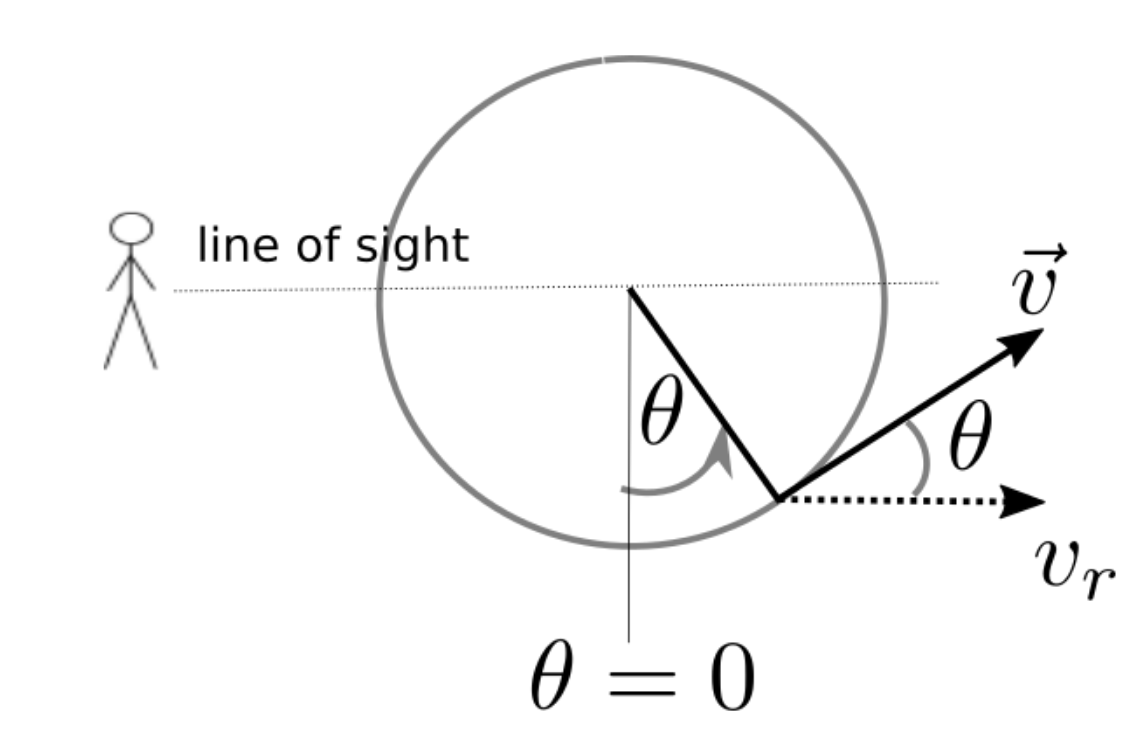
\includegraphics[scale=0.3]{media/vrmod.png}
\end{frame}
}

{
\setbeamercolor{background canvas}{bg=yellow}
\begin{frame}
\label{riktigm2}
\begin{columns}
\column{0.5\textwidth}
\clastpagebutton{stat3}
Helt riktig. Stjerna skal gå en hel rundt på $2\pi$ i løpet av perioden $P$, dermed er vinkelhastigheten $\frac{2\pi}{P}$. Ganger vi dette med tiden $t$ som har gått så får vi vinkelen. Setter vi dette inn i vårt forrige resultat så har vi
\[
v_r(t)=v_*\cos{\frac{2\pi}{P}t}
\]
På figuren hadde vi definert når vinkelen $\theta$ er 0. Vi går nå bort ifra denne definisjonen og sier at ved tiden $t=t_0$ så er $\theta=0$. Vi definerer altså isteden et tidspunkt $t_0$ der vinkelen er 0:
\[
v_r(t)=v_*\cos{\frac{2\pi}{P}(t-t_0)}
\]
\column{0.5\textwidth}
Hvis vi definerer $t_0$ på denne måten, hvor på kurven er vi ved $t=t_0$??
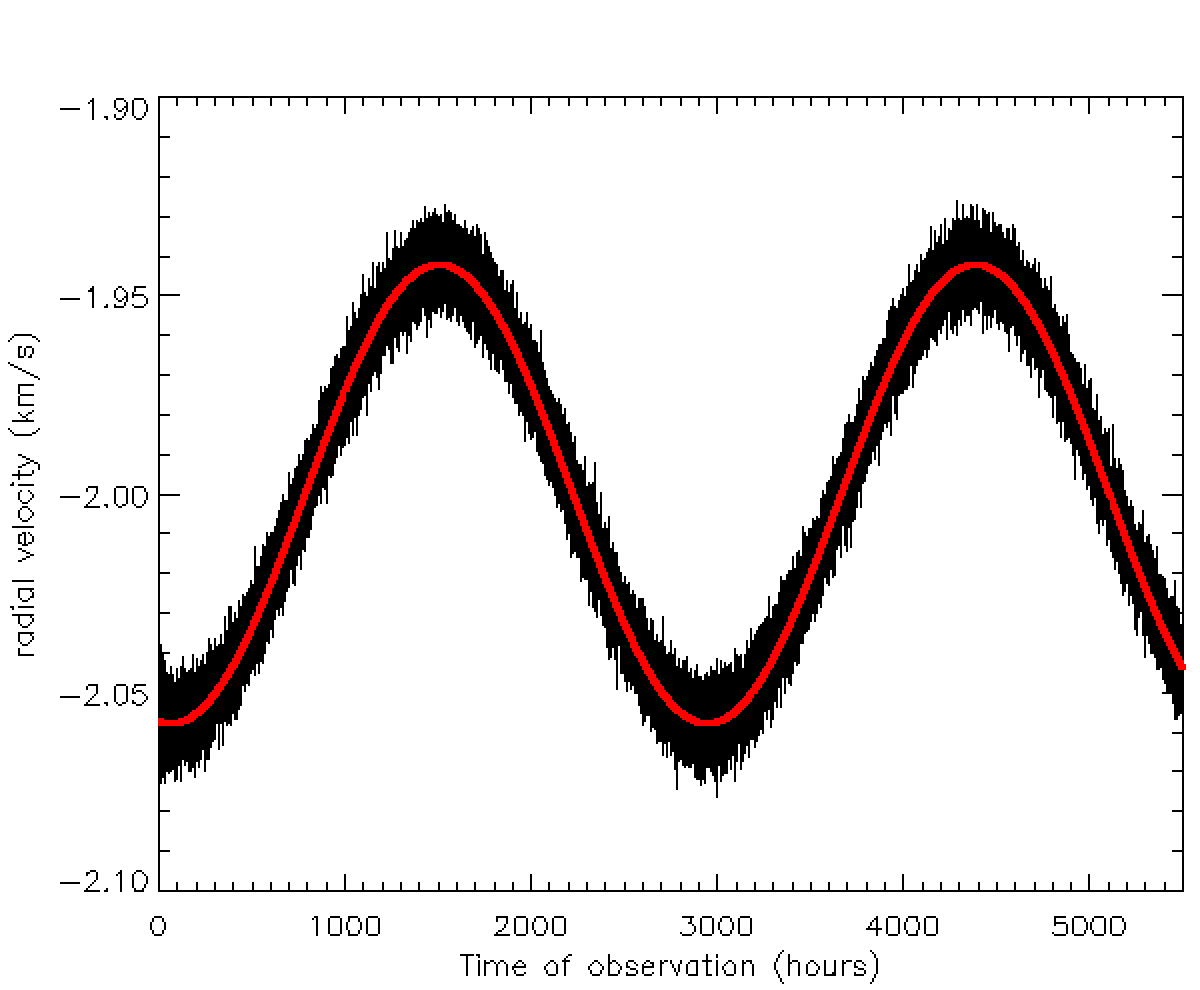
\includegraphics[scale=0.25]{media/vr_noisy.png}\\
\vspace*{0.5cm}
{\bf Tenk før du blar om (maks 1 min)!}
\hyperlink{red_sikker}{\pagebutton{Neste side}}
\end{columns}
\end{frame}
}

{
\setbeamercolor{background canvas}{bg=red}
\begin{frame}
\label{red_sikker}
\hyperlink{riktigm2}{\pagebutton{\small Forrige side}}
\textcolor{yellow}{\Huge\bf Er du helt sikker på at du tenkte deg godt om nå??? Ikke no' juks her! Hvis du ikke hadde tenkt deg om, gå tilbake til forrige side og tenk! Hvis du hadde tenkt: beklager så mye, det var absolutt ikke meningen å insinuere at du ikke følger instrukser.}
\hyperlink{stat4}{\pagebutton{Neste side}}
\end{frame}
}


\begin{frame}
\label{stat4}
\begin{columns}
\column{0.5\textwidth}
\lastpagebutton{riktigm2}
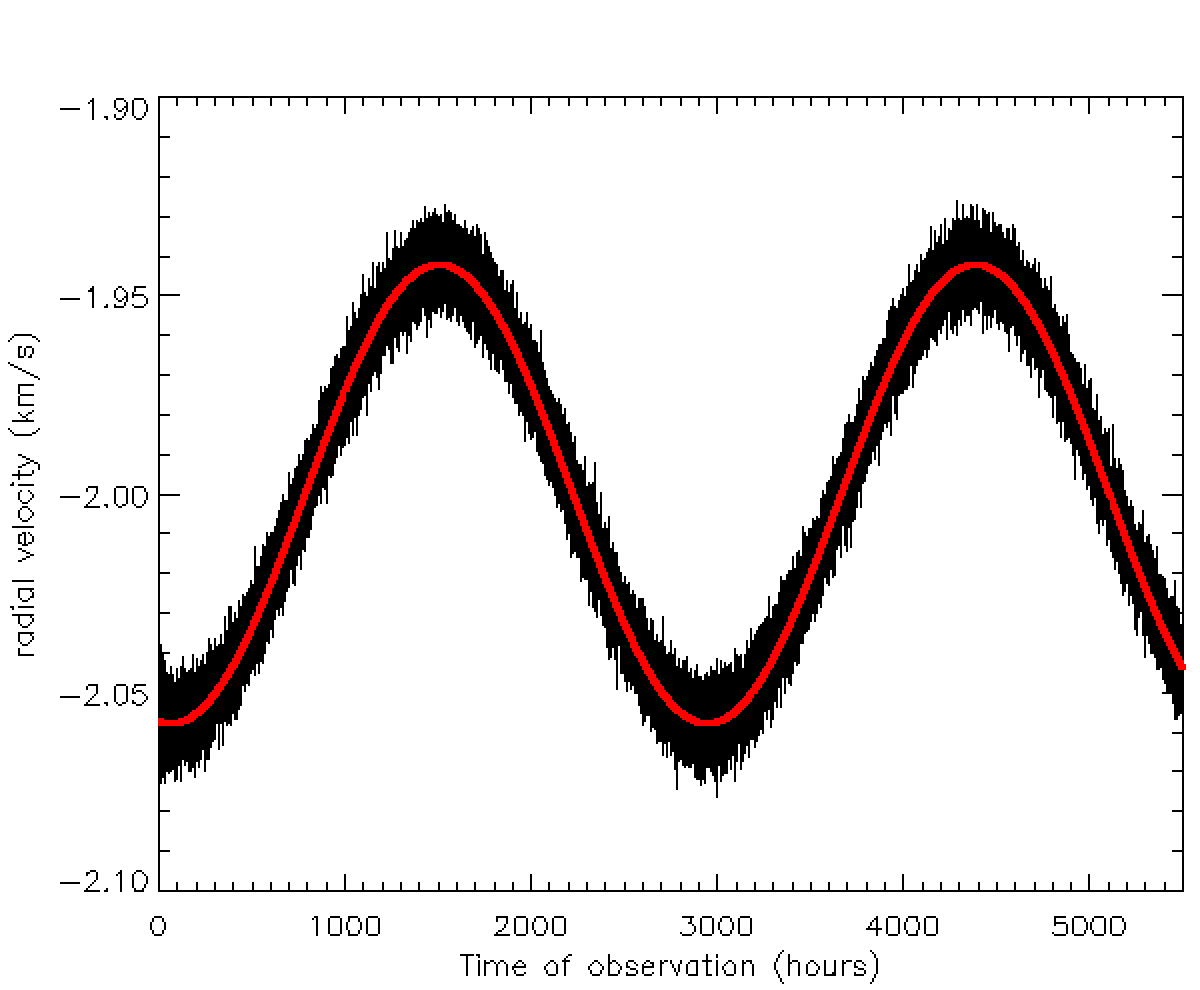
\includegraphics[scale=0.25]{media/vr_noisy.png}\\
Hvis vi ser på uttrykket:
\[
v_r(t)=v_*\cos{\frac{2\pi}{P}(t-t_0)}
\]
så ser vi at ved $t=t_0$ så er $v_r=v_*$, altså radialhastigheten er lik den fulle banehastigheten.
\column{0.5\textwidth}

 Da er radialhastigheten maksimal, altså er vi på toppen av kurven.
 Dette skulle du huske fra diskusjonen i forrige forelesning: dette er punktet hvor stjernen er på vei bort fra oss langs vår synslinje og hele banehastigheten er i radialhastigheten uten noen tangensialkomponent (hvis vi antar at inklinasjonen er $90^\circ$!). Dette var punktet B på figuren i forrige forelesning. Repeter litt hvis du er usikker. 
\hyperlink{stat5}{\pagebutton{Neste side}}
\end{columns}
\end{frame}


{
\setbeamercolor{background canvas}{bg=aquamarine}
\begin{frame}
\label{stat5}
\begin{columns}
\column{0.5\textwidth}
\lastpagebutton{stat4}
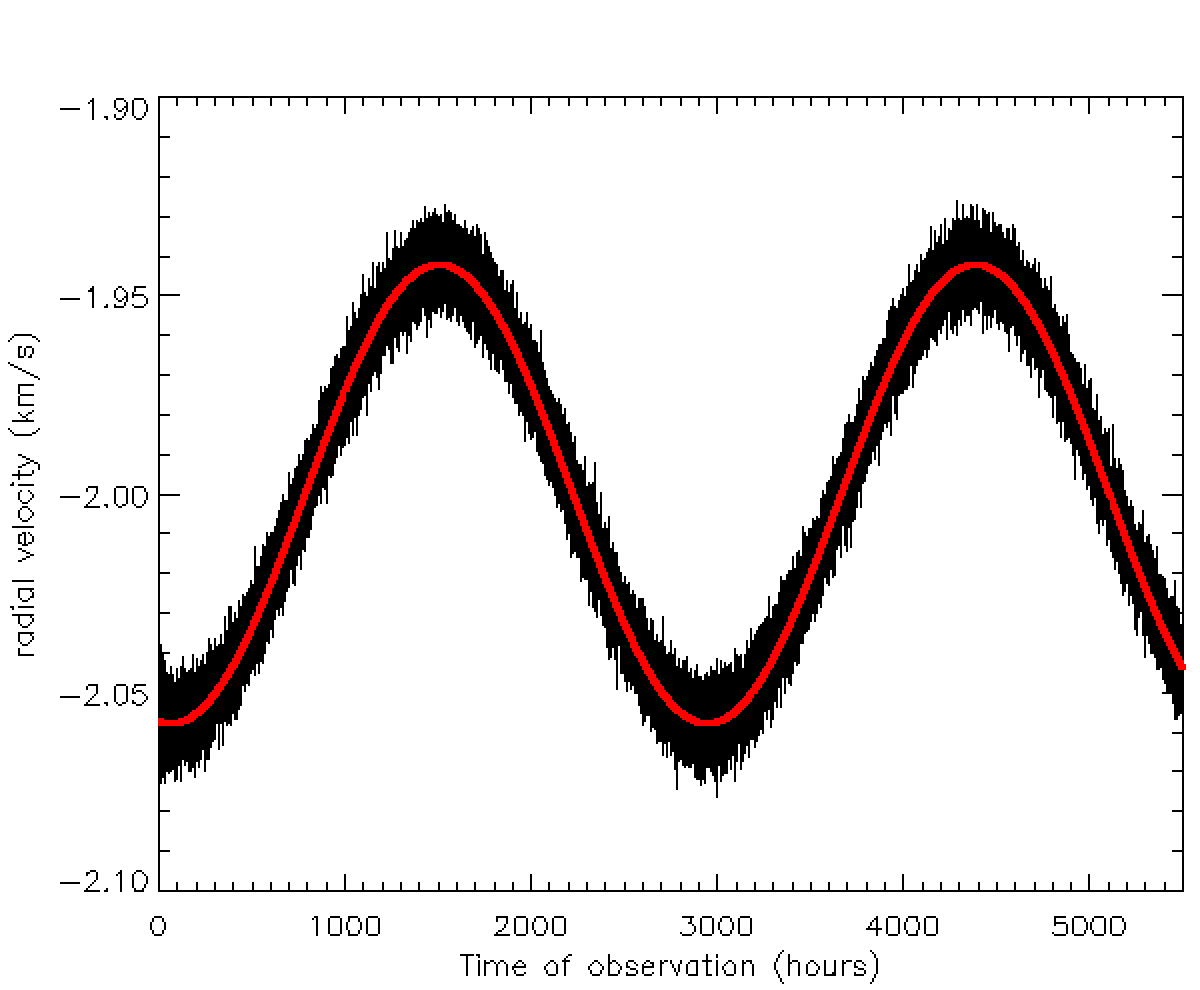
\includegraphics[scale=0.25]{media/vr_noisy.png}\\
{\small
\[
v_r(t)=v_*\cos{\frac{2\pi}{P}(t-t_0)}
\]

Vi har nå et uttrykk for hvordan kurven skal se ut hvis vi ikke har støy, uttrykt ved banehastigheten $v_*$, omløpsperioden $P$ og tidspunktet $t_0$ når kurven har første topp-punkt. Problemet er bare at vi ikke kjenner noen av disse 3 parameterene.
} 
\column{0.5\textwidth}
{\small
 \textcolor{red}{\bf Det er akkurat disse størrelsene vi ønsker å finne!!}.
Hvis vi finner $v_*$ og $P$ så kan vi estimere massen til planeten slik som i forrige forelesning. Men vi har altså en støyete kurve som gjør det vanskelig å lese av $v_*$ og $P$, samtidig har vi en analytisk modell som sier hvordan den underliggende støyfrie kurven skal se ut, dersom vi kjenner $v_*$ og $P$. \textcolor{red}{Det store spørsmålet nå er, hvordan kan vi bruke den analytiske modellen vår, sammen med den observerte støyete kurven til å finne gode estimater av tallene $v_*$ og $P$?} Diskuter med medstudenter, og ikke gå videre før du har tenkt {\bf godt} gjennom problemstillingen (3 min)!!!
}
\hyperlink{stat6}{\pagebutton{Neste side}}
\end{columns}
\end{frame}
}


\begin{frame}
\label{stat6}
\lastpagebutton{stat5}
{\Huge
Det var noen setninger på den forrige siden som er ganske så uforstålige hvis du ikke leser de flere ganger og tenker deg godt om. \textcolor{red}{Ta et skritt tilbake og se om du faktisk forstod hva som stod der, ok?} Når du har forstått hva som stod der, har du tenkt litt? Har du fått noen ideer? Tenk litt til før du går videre!
}
\hyperlink{blue_nytema3}{\pagebutton{Neste side}}
\end{frame}


\renewcommand{\headline}{\small Minste kvadraters metode}
{
\setbeamercolor{background canvas}{bg=blue}
\begin{frame}
\label{blue_nytema3}
\hyperlink{stat6}{\pagebutton{\small Forrige side}}
\nytemaside{stat}
\hyperlink{stat7}{\pagebutton{Vi tar kaffepause ved neste tema, litt til først!}}
\end{frame}
}

\begin{frame}
\label{stat7}
\lastpagebutton{stat6}\label{minstekvad}
\begin{columns}
\column{0.5\textwidth}
Har du hørt om {\it minste kvadraters metode?}. Metoden som går ut på å {\bf minimalisere forskjellen mellom modellen og dataene?}
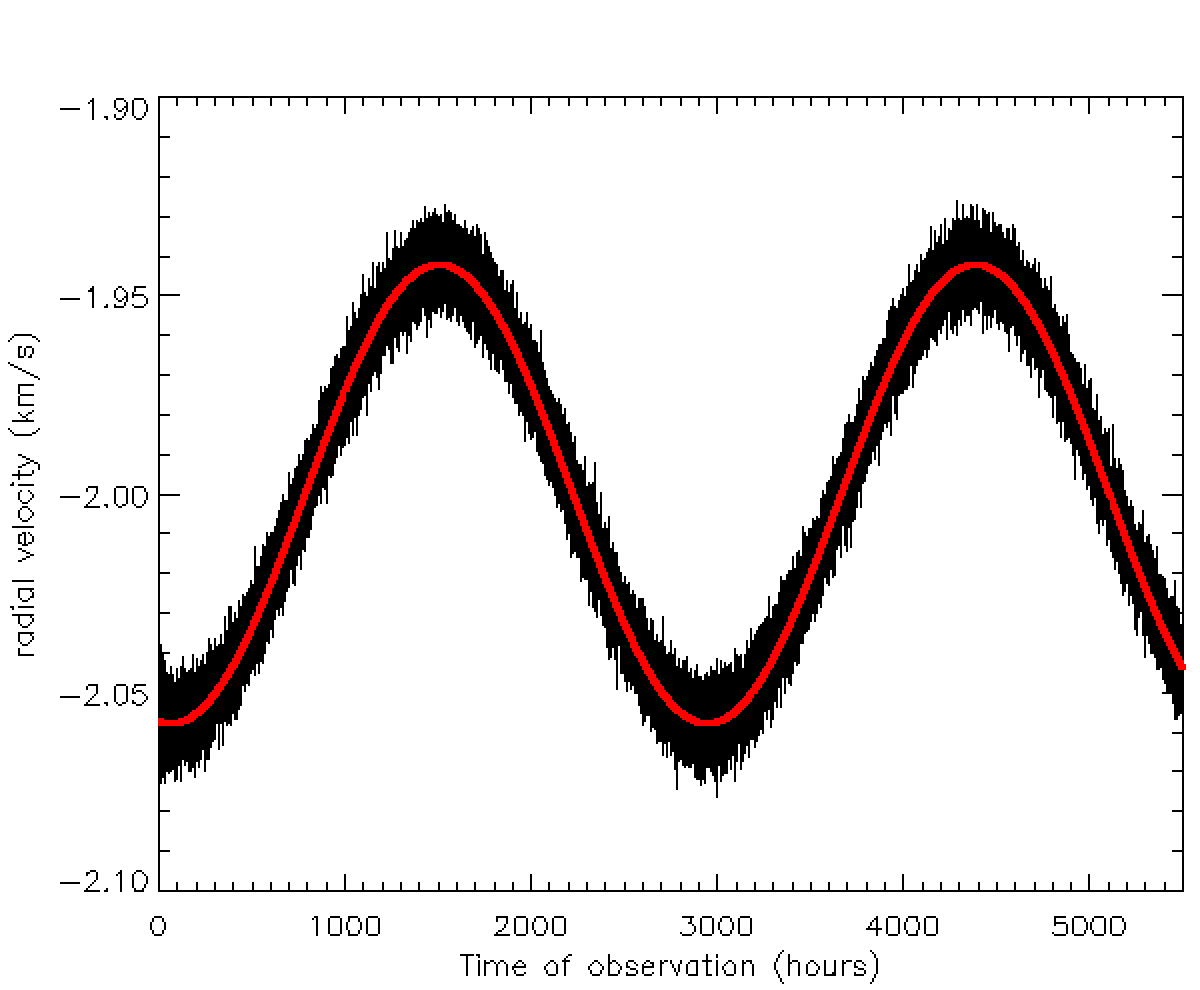
\includegraphics[scale=0.22]{media/vr_noisy.png}\\
Vi skal finne den røde linja som passer best til de observerte dataene med støy.
\column{0.5\textwidth}
 Vi vet at de røde linjene vi kan tegne, alle må følge:
\[
v_r(t)=v_*\cos{\frac{2\pi}{P}(t-t_0)}
\]
Vi kan endre på den røde linja ved å endre på verdiene for $v_*$, $P$ og $t_0$. \textcolor{red}{Minste kvadraters metode sier oss altså å justere modellen (den røde linja), dvs. endre de ukjenten parameterene $v_*$, $P$ og $t_0$, helt til vi finner den modell-linja som gir minst forskjell mellom modellen og den observerte kurven.}
\hyperlink{stat8}{\pagebutton{Neste side}}
\end{columns}
\end{frame}


\begin{frame}
\label{stat8}
\lastpagebutton{stat7}
\begin{columns}
\column{0.5\textwidth}
{\it Minste kvadraters metode} går altså ut på å {\bf minimalisere forskjellen mellom modellen og dataene:}
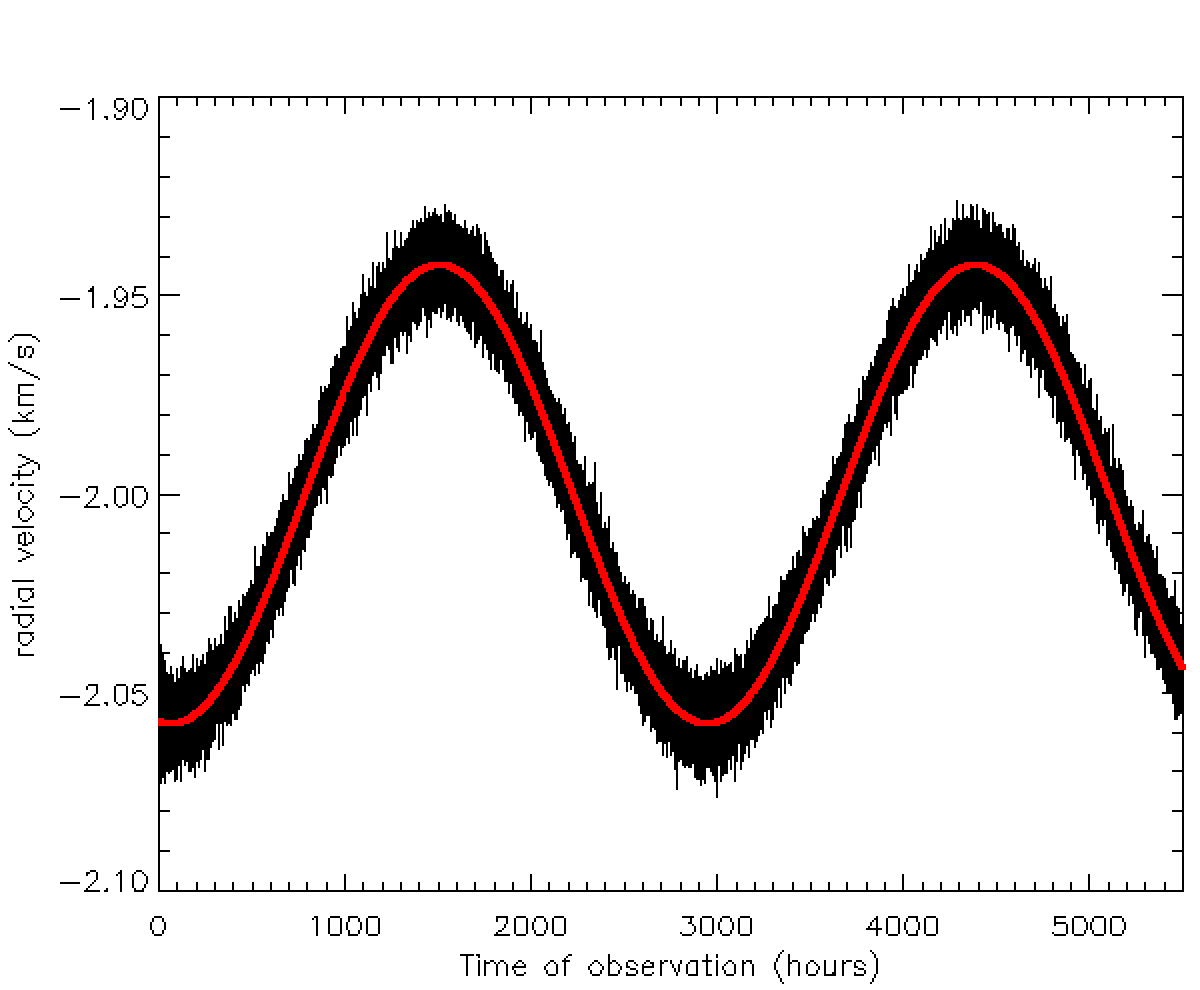
\includegraphics[scale=0.22]{media/vr_noisy.png}\\
 Der vi vet at modellen vår er gitt ved:
\[
v_r(t)=v_*\cos{\frac{2\pi}{P}(t-t_0)}
\]
\column{0.5\textwidth}
Men hvordan defineres {\bf den minste forsjellen?}. Det er rett og slett {\bf forskjell} slik vi vanligvis omtaler en forskjell: \textcolor{red}{datakurven minus modellkurven. Men vi opphøyer denne forsjellen i annen potens}, derav navnet {\bf minste kvadrat}. Dette er for å få absoluttverdien, det er ikke viktig om forskjellen er negativ eller positiv. Det finnes også en statistisk begrunnelse for å ta kvadratet, denne kommer snart.
\hyperlink{stat8b}{\pagebutton{Neste side}}
\end{columns}
\end{frame}


\begin{frame}
\label{stat8b}
\lastpagebutton{stat8}
\begin{columns}
\column{0.5\textwidth}
\small
Vi skal altså lage oss mange forskjellige røde kurver med forskjellige tallverdier for $P$, $v_*$ og $t_0$
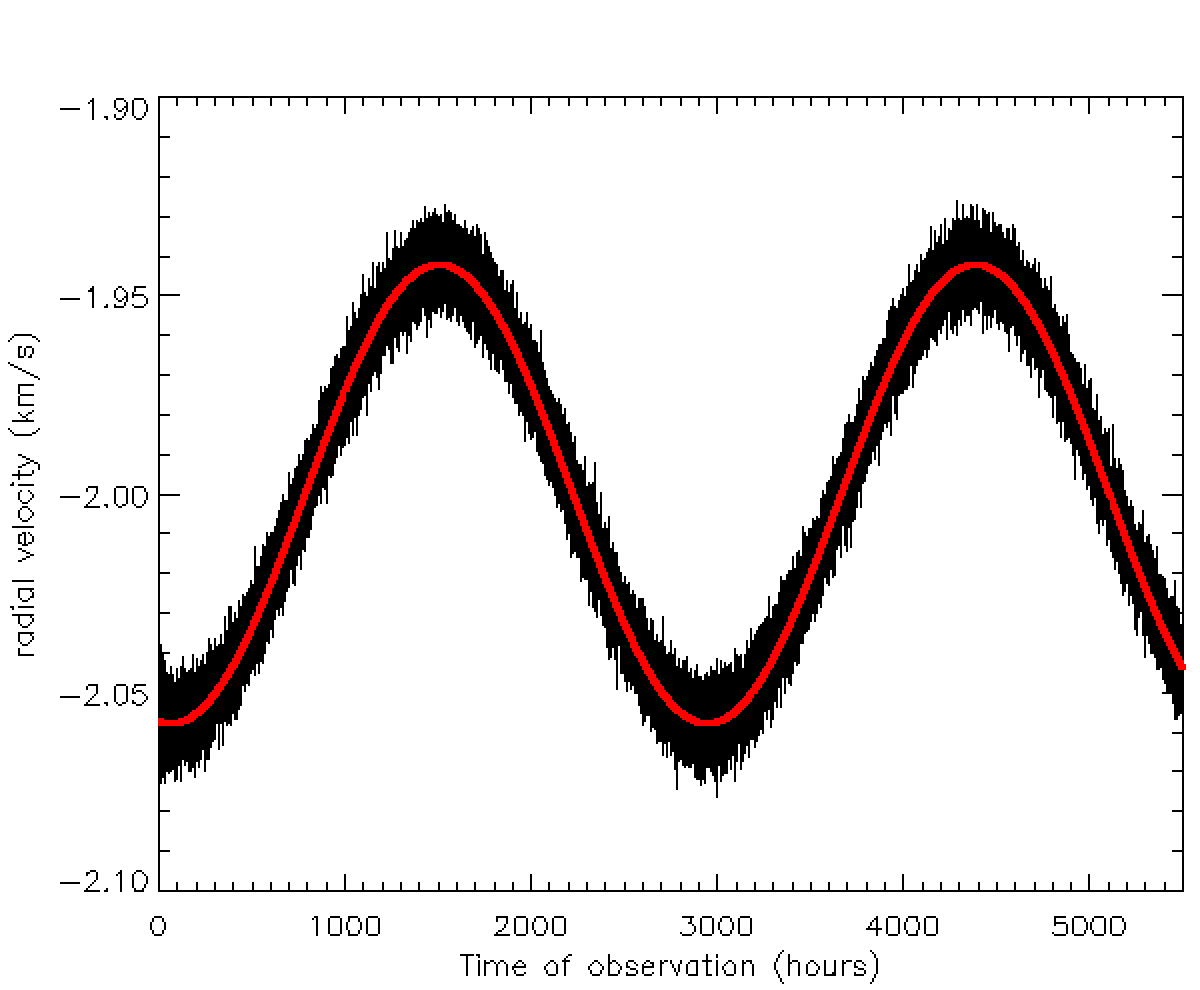
\includegraphics[scale=0.22]{media/vr_noisy.png}\\
\[
v_r^\mathrm{mod}(t)=v_*\cos{\frac{2\pi}{P}(t-t_0)}
\]
helt til vi finner en som gir oss den minste mulige kvadratforskjellen. Rent matematisk skal vi altså summere kvadratforskjellen over alle målepunktene våre, dvs over alle observerte tidspunkter $t_i$.
\column{0.5\textwidth}
\small
 Tidspunktet for observasjon nr. $i$ er derfor $t_i$ og vi har totalt $N$ slike observasjoner. Da få vi at kvadratforskjellen er gitt ved:
\begin{align*}
&\Delta(v_*, P, t_0) = \\
&\sum_{i=1}^{N} \left( v_r^{\mathrm{obs}} (t_i) - v_r^{\mathrm{mod}} (t_i, v_*, P, t_0) \right)^{2}
\end{align*}
der vi ser at $\Delta$ altså er en funksjon av de ukjente parameterene $P$, $v_*$ og $t_0$. Her er $v_r^\mathrm{obs}$ den observerte sorte kurven og $v_r^\mathrm{mod}$ er den røde modellkurven. Vi skal altså finne de parameterene $P$, $v_*$ og $t_0$ som minimaliserer $\Delta$. Dette vil være de tallene $P$, $v_*$ og $t_0$ som passer best til dataene og de vi skal bruke videre til å finne massen.
\hyperlink{pause}{\pagebutton{Neste side}}
\end{columns}
\end{frame}

{
\setbeamercolor{background canvas}{bg=cyan}
\begin{frame}
\label{pause}
\hyperlink{stat8b}{\pagebutton{\small Forrige side}}
{\Huge
\centerline{TID FOR KAFFEPAUSE!!!}
\centerline{
\includegraphics[scale=4]{media/drink-coffee.png}}\\
Ut å strekke på bena. Inn med litt koffein...\\
{\small Og kanskje kan du tillate deg en sjokoladebit? Men ikke si det høyt!}\\
\vspace*{0.5cm}
Ihvertfall 10 min...
}\\
\vspace*{0.5cm}
\hyperlink{blue_nytema4}{\pagebutton{Jeg lover, jeg har tatt pause og er klart til å fortsette}}
\end{frame}
}

\renewcommand{\headline}{\small Støy i data:statistikk}
{
\setbeamercolor{background canvas}{bg=blue}
\begin{frame}
\label{blue_nytema4}
\hyperlink{stat8b}{\pagebutton{\small Forrige side}}
\nytemaside{tips}
\hyperlink{red_stat9}{\pagebutton{Sett igang med nytt tema!}}
\end{frame}
}


{
\setbeamercolor{background canvas}{bg=red}
\begin{frame}
\label{red_stat9}
\lastpagebutton{stat8b}\label{stat}
\large
Men er dette virkelig det beste vi kan gjøre? Det blir jo noen unøyaktigheter i verdiene for $P$, $v_*$ og $t_0$ som vi får med denne metoden. Hvor presise resultatene våre er avhenger av hvor kraftig støy det er. Hvis vi nå skulle kjenne noen egenskaper til støyen, noe vi normalt gjør, kan vi da finne en mer sofistikert metode som gir oss bedre estimater? For å finne ut av dette, la oss dykke litt ned i {\Large \bf statistikken her...}

\includegraphics[scale=0.3]{media/diving.png}\\
\hyperlink{stat10}{\pagebutton{Neste side}}
\end{frame}
}





\begin{frame}
\label{stat10}
\lastpagebutton{red_stat9}
Normalt kan vi anta Gaussisk støy. Dvs at vi kan skrive hastigheten $v_r$ i observasjon nr. $i$ som
\[
v_r^\mathrm{obs}(t_i)=v_r^\mathrm{real}(t_i)+\delta v_i
\]
der \textcolor{blue}{$v_r^\mathrm{real}$ er det faktiske hastighetskurven} som du hadde sett hvis det ikke hadde vært støy i instrumentet og \textcolor{blue}{$\delta v_i$ er støy i observasjon $i$}. Hvis støyen er Gaussisk så betyr det at $\delta v_i$ er et tilfeldig tall trukket fra en Gaussisk sannsynlighetsfordeling. Normalt er denne med middelverdi 0 slik at hvis man hadde en uendelig mengde observasjoner av det samme datapunktet så vill du i middel fått den faktiske verdien. I tillegg kan man ofte måle standardavviket til fordelingen, vi kaller denne $\sigma_n$ der $n$ står for {\it noise}. Gitt at denne er kjent, \textcolor{red}{skriv ned sannsynlighetsfordelingen $P(\delta v_i)$, dvs. sannsynligheten for at vi ved en gitt observasjon får en verdi $\delta v_i$ for støyen}.\\
{\bf Er du klar?} {\bf Har du et forslag til sannsynlighetsfordeling? Er du usikker, ta gjerne en kikk tilbake til del 1A for å reptere litt om Gaussiske sannsynlighetsfordeling. Du kommer til å få bruk for dette igjen, så gjør det med en gang, så du er klar til å gå videre!}.
\hyperlink{stat11}{\pagebutton{\small Neste side (bare når du har et forslag til sannsynlighetsfordeling)}}
\end{frame}


\begin{frame}
\label{stat11}
\lastpagebutton{stat10}
I del 1A lært vi at en Gaussisk sannsynlighetsfordeling for en stokastisk variabel $x$ med gjennomsnittsverdi $\mu$ og standardavvik $\sigma$ er gitt ved
\[
P(x) = \frac{1}{\sqrt{2\pi}\sigma}e^{-\frac{1}{2}\frac{(x-\mu)^2}{\sigma^2}}
\]
Hvis middelverdien for støyen er 0, noe den ofte er, og standardavviket er $\sigma_n$, så bli jo det da rett og slett:
\[
P(\delta v_i) = \frac{1}{\sqrt{2\pi}\sigma_n}e^{-\frac{1}{2}\frac{\delta v_i^2}{\sigma_n^2}}
\]
som igjen er en {\it sannsynlighetstetthet}, dvs at vi må gange med et intervall av mulige verdier for støyen $\delta v_i$ for å få en faktisk sannsynlighet.
\hyperlink{stat12}{\pagebutton{\small Neste side}}
\end{frame}

\begin{frame}
\label{stat12}
\lastpagebutton{stat11}
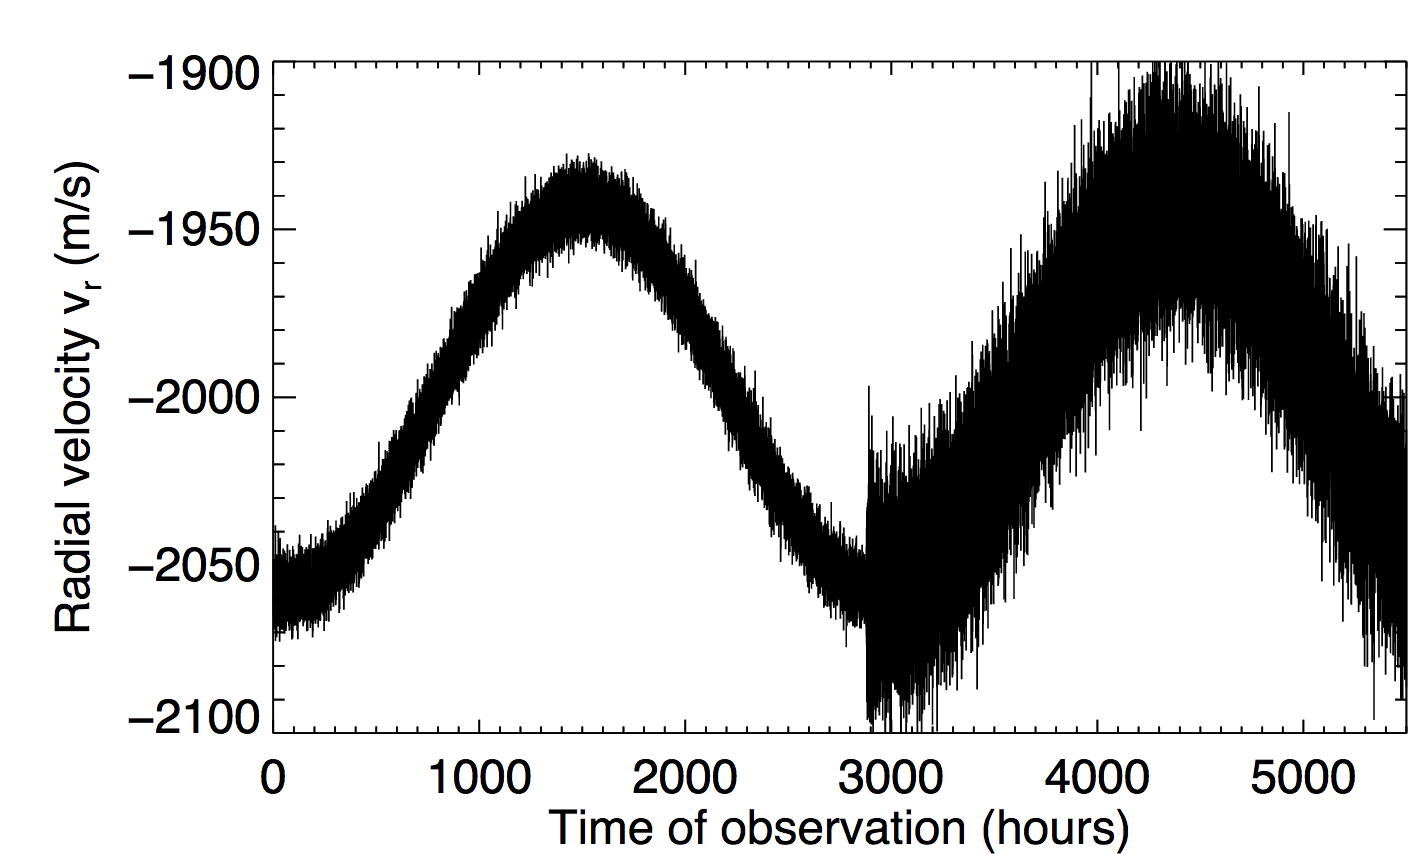
\includegraphics[scale=0.3]{media/twosigma.png}\\
På figuren ser du observasjoner av en hastighetskurve med to forskjellige teleskoper, et med betydelig høyere støynivå enn det andre. Dermed er standardavviket $\sigma_n$ for støyen også forskjellig. Omtrent hva er $\sigma_n$ for hver av disse instrumentene? La oss kalle observasjonene til venstre med minst støy for A og de til høyre med mest støy for B.\\
\hyperlink{feiln}{\choicebutton{\small $\sigma_n^A\approx 1930$m/s og $\sigma_n^B\approx 1900$m/s}}\ \hyperlink{feiln}{\choicebutton{\small $\sigma_n^A\approx 140$m/s og $\sigma_n^B\approx 200$m/s}}\ \hyperlink{feiln}{\choicebutton{\small $\sigma_n^A\approx 30$m/s og $\sigma_n^B\approx 80$m/s}}\ \hyperlink{feiln}{\choicebutton{\small $\sigma_n^A\approx 15$m/s og $\sigma_n^B\approx 40$m/s}}\ \hyperlink{riktign}{\choicebutton{\small $\sigma_n^A\approx 7$ m/s og $\sigma_n^B\approx 20$m/s}}
\end{frame}



{
\setbeamercolor{background canvas}{bg=black}
\begin{frame}
\label{feiln}
\lastpagebutton{stat12}
\textcolor{white}{\small Det var ikke helt riktig. Under ser du en zoom av området rundt toppen av kurven til venstre (vi kunne ha tatt hvor som helst på kurven). Den røde linjen er observasjonen du hadde hatt uten støy, dvs. når støyen er 0. Utsalgene over og under er når du får positive eller negative verdier for støyen $\delta v_i$. Husker du at 95\% av verdiene for en Gaussisk fordeling skal ligge innenfor $2\sigma$? {\bf Hvis ikke, så er det svært viktig at du går tilbake til del 1A da du har glemt viktig kunnskap som du trenger videre}. Ta nå et papir, tegn en Gaussisk sannsynlighetsfordeling med forskjellige verdier for $\delta v_i$ på x-aksen, med da 0 i midten siden gjennomsnittsverdien for denne Gaussiske fordelingen er 0. Tegn inn $1\sigma$ og $2\sigma$ (gjerne med hjelp av kurver fra del 1A) og sammenlikn med figuren under. Gå nå tilbake og gjør et nytt forsøk.}\\
\centerline{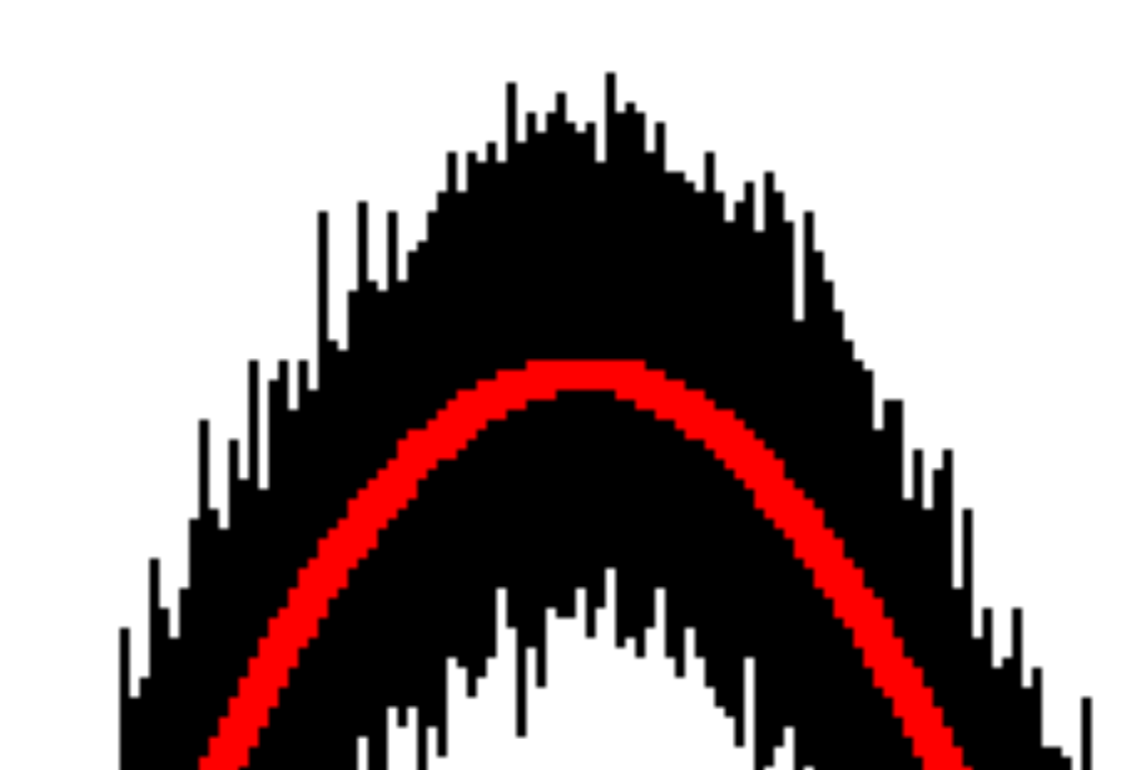
\includegraphics[scale=0.3]{media/noise_zoom.png}}
\end{frame}
}

{
\setbeamercolor{background canvas}{bg=yellow}
\begin{frame}
\label{riktign}
\clastpagebutton{stat12}
Flott! Du fikk det til. Det betyr at du forstår hva det betyr at støyen er Gaussisk fordelt og hva en Gaussisk fordeling er. Hvis du nå likevel er litt usikker, ta en titt på \href{https://www.uio.no/studier/emner/matnat/astro/AST2000/h20/undervisningsressurser/interaktive-forelesningsnotater/1c/videoer/video1c_7.mp4}{denne videoen}.
\hyperlink{stat13}{\pagebutton{Neste side}}
\end{frame}
}

\begin{frame}
\label{stat13}
\lastpagebutton{riktign}
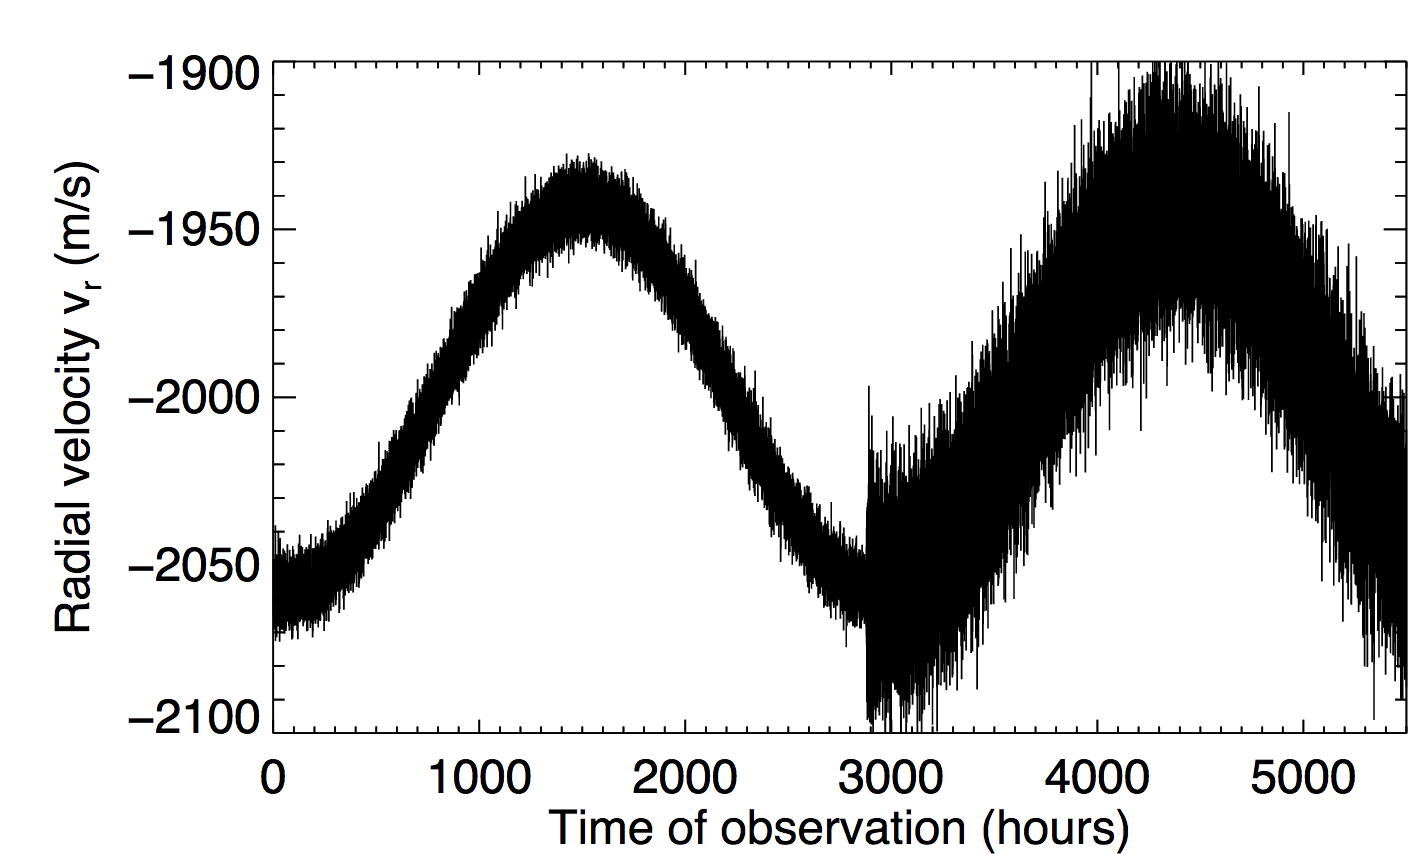
\includegraphics[scale=0.25]{media/twosigma.png}\\
{\small 
Men hva skal vi gjøre i en slik situasjon når støyen varierer med tiden? Hvis vi bruker vanlig minste kvadraters metode her, så behandler vi dataene av dårlig kvalitet på samme måte som dataene av god kvalitet, kan det være riktig? Vi kan vel ikke få et optimalt godt estimat av modellen vår på den måten? Kan du tenkte deg hvordan vi kan gjøre en liten modifikasjon av minste kvadraters metode
\[
\Delta(v_*, P, t_0) = \sum_{i=1}^N\left(v_r^\mathrm{obs}(t_i)-v_r^\mathrm{mod}(t_i, v_*, P, t_0)\right)^2
\]
for å ta hensyn til at standardavviket til støyen ikke alltid er den samme?
{\bf Tenk deg om (1 min) før du går videre!}
}
\hyperlink{stat13b}{\pagebutton{Neste side}}
\end{frame}


\begin{frame}
\label{stat13b}
\lastpagebutton{stat13}
La oss se om vi kan utlede hva som er den beste måten å gjøre dette på!\\
La oss fortsette med statitsikken. Vi fant at sannsynligheten for støyen i observasjon $i$ er gitt ved
\[
P(\delta v_i) = \frac{1}{\sqrt{2\pi}\sigma_n}e^{-\frac{1}{2}\frac{\delta v_i^2}{\sigma_n^2}}
\]
Hvis vi antar at standardavviket til støyen endrer seg for hver observasjon $i$ og at standardavviket for støyen for observasjon nr. $i$ er gitt ved $\sigma_i$, så blir vel den modifiserte sannsynligheten
\[
P(\delta v_i) = \frac{1}{\sqrt{2\pi}\sigma_i}e^{-\frac{1}{2}\frac{\delta v_i^2}{\sigma_i^2}}
\]
Enig? \hyperlink{riktig_ja}{\choicebutton{Ja}}\ \hyperlink{feil_nei}{\choicebutton{Nei}}
\end{frame}



{
\setbeamercolor{background canvas}{bg=black}
\begin{frame}
\label{feil_nei}
\lastpagebutton{stat13b}
\textcolor{white}{
\Large
Hvorfor ikke????
Er du usikker, spør foreleser!
}
\hyperlink{riktig_ja}{\pagebutton{Neste side}}
\end{frame}
}

{
\setbeamercolor{background canvas}{bg=yellow}
\begin{frame}
\label{riktig_ja}
\clastpagebutton{stat13b}
Flott, da kan vi gå videre. Vi har altså
\[
P(\delta v_i) = \frac{1}{\sqrt{2\pi}\sigma_i}e^{-\frac{1}{2}\frac{\delta v_i^2}{\sigma_i^2}}
\]
for sannsynligheten i et gitt tidspunkt $i$. Men hva er sannsynligheten for at vi får et helt sett med verdier \{$\delta v_0$, $\delta v_1$, $\delta v_2$, ..., $\delta v_N$\}? Dvs. hva er f.eks. sannsynligheten for at vi får akkurat alle de støyverdiene som vi ser på figuren for alle tidspunkter $i$? ({\bf Hint: lov om multiplikasjon av sannsynlighet})\\
{\bf Ikke gå til neste side før du har et forslag til sannsynlighetsfordeling for $P(\delta v_0, \delta v_1, \delta v_2, ..., \delta v_N)$}
\hyperlink{stat14}{\pagebutton{Neste side}}
\end{frame}
}



\begin{frame}
\label{stat14}
\lastpagebutton{riktig_ja}
Nettopp ja, loven om multiplikasjon av sannsynligheter, vi ganger sammen sannsynligheten for støyen hvert tidspunkt $i$ for å få den totale sannsynligheten for alle støyverdiene i alle N observasjonstidspunkter (hvis vi går tilbake til eksemplet vårt i del 1A så kan du jo tenke deg at den første støyverdien er høyden til en tilfeldig person, den andre er IQ-en til en tilfeldig person, den tredje er vekta til en tilfeldig person, etc. Ved å gange sammen sannsynlighetene kan du finne sannsynligheten for at en person har et gitt sett med verdier for disse 3 egenskapene, akkurat som vi nå kan finne sannsynligheten for at støyen i hvert observasjonspunkt har et gitt sett med verdier).
\[
P(\delta v_0, \delta v_1, \delta v_2, ..., \delta v_N)) = \prod_{i=1}^N\frac{1}{\sqrt{2\pi}\sigma_i}e^{-\frac{1}{2}\frac{\delta v_i^2}{\sigma_i^2}}
\]
\hyperlink{stat15}{\pagebutton{Neste side}}
\end{frame}


\begin{frame}
\label{stat15}
\lastpagebutton{stat14}
Ser du at vi kan skrive om på følgende måte...dette var uttrykket vår:
\[
P(\delta v_0, \delta v_1, \delta v_2, ..., \delta v_N)) = \prod_{i=1}^N\frac{1}{\sqrt{2\pi}\sigma_i}e^{-\frac{1}{2}\frac{\delta v_i^2}{\sigma_i^2}}
\]
og ved å skrive ut faktorene etterhverandre og bruke det vi kan om eksponenter, så kan vi skrive det som
\[
P(\delta v_0, \delta v_1, \delta v_2, ..., \delta v_N) = \left(\frac{1}{\sqrt{2\pi}}\right)^N\frac{1}{\prod_{i=1}^N\sigma_i}e^{-\frac{1}{2}\sum_{i=1}^N\frac{\delta v_i^2}{\sigma_i^2}}
\]
Kan du se at det stemmer? Hvis ikke, skriv dette ut på papir og bruk loven om at man kan summe eksponentene i et produkt. {\bf Ser du det? Hvis ikke spør foreleser!}
\hyperlink{stat16}{\pagebutton{Neste side}}
\end{frame}



\begin{frame}
\label{stat16}
\lastpagebutton{stat15}
Hvis du går noen sider tilbake vil du se at vi skrev:
\[
v_r^\mathrm{obs}(t_i)=v_r^\mathrm{real}(t_i)+\delta v_i
\]
Dette skriver vi om til
\[
\delta v_i = v_r^\mathrm{obs}(t_i)-v_r^\mathrm{real}(t_i)
\]
og setter inn for $\delta v_i$ i uttrykket vårt. Da får vi
\[
P(\delta v_0, \delta v_1, \delta v_2, ..., \delta v_N) = \left(\frac{1}{\sqrt{2\pi}}\right)^N\frac{1}{\prod_{i=1}^N\sigma_i}e^{-\frac{1}{2}\sum_{i=1}^N\frac{(v_r^\mathrm{obs}(t_i)-v_r^\mathrm{real}(t_i))^2}{\sigma_i^2}}
\]
Målet vår er å finne en modell for $v_r^\mathrm{real}(t_i)$, dvs. en modell $v_r^\mathrm{mod}(t_i)$ som vi setter som vårt estimat av den reelle hastighetskurven. Hvis du kikker på uttrykket, begynner du å ane hvor minste kvadraters metode kommer fra? Og begynner du ane hvordan den kan modifiseres?
\hyperlink{stat17}{\pagebutton{Neste side}}
\end{frame}


\begin{frame}
\label{stat17}
\lastpagebutton{stat16}
Hvis vi setter inn modellen vår som den virkelige kurven så blir det:
\[
P(\delta v_0, \delta v_1, \delta v_2, ..., \delta v_N) = \left(\frac{1}{\sqrt{2\pi}}\right)^N\frac{1}{\prod_{i=1}^N\sigma_i}e^{-\frac{1}{2}\sum_{i=1}^N\frac{(v_r^\mathrm{obs}(t_i)-v_r^\mathrm{mod}(t_i))^2}{\sigma_i^2}}
\]
hvor vi vet at $v_r^\mathrm{mod}(t_i)$ inneholder de ukjente parameterene $v_*$, $P$ og $t_0$ som vi ønsker å finne. Vi ønsker altså å finne den modellen, dvs. de parameterene $v_*$, $P$ og $t_0$, som gir den største mulige sannsynligheten for å observere den kurven, dvs. det sett med verdier $\delta v_0, \delta v_1, \delta v_2, ..., \delta v_N$ som vi faktisk observerer. Vi ønsker altså å finne de verdiene for $v_*$, $P$ og $t_0$ som maksimaliserer sannsynligheten $P(\delta v_0, \delta v_1, \delta v_2, ..., \delta v_N)$. Hvordan kan vi skrive dette matematisk litt enklere??
\hyperlink{stat18}{\pagebutton{Neste side}}
\end{frame}

\begin{frame}
\label{stat18}
\lastpagebutton{stat17}
Vi har
\[
P(\delta v_0, \delta v_1, \delta v_2, ..., \delta v_N) = \left(\frac{1}{\sqrt{2\pi}}\right)^N\frac{1}{\prod_{i=1}^N\sigma_i}e^{-\frac{1}{2}\sum_{i=1}^N\frac{(v_r^\mathrm{obs}(t_i)-v_r^\mathrm{mod}(t_i))^2}{\sigma_i^2}}
\]
som skal maksimaliseres. Er du enig i at dette er identisk med å maksimalisere eksponenten her? Og siden det står et minustegn i eksponenten, er du enig i at vi da skal {\bf minimalisere} det som kommer etter minustegnet? Tenk to ganger for å sjekke om du er enig!
\hyperlink{stat19}{\pagebutton{Neste side}}
\end{frame}


\begin{frame}
\label{stat19}
\lastpagebutton{stat18}
Er vi dermed enige om at for å maksimalisere sannsynligheten, så må vi {\bf minimalisere}
\[
\sum_{i=1}^N\frac{(v_r^\mathrm{obs}(t_i)-v_r^\mathrm{mod}(t_i))^2}{\sigma_i^2}
\]
Denne størrelsen pleier vi å kalle $\chi^2$, dvs.
\[
\chi^2 = \sum_{i=1}^N\frac{(v_r^\mathrm{obs}(t_i)-v_r^\mathrm{mod}(t_i))^2}{\sigma_i^2}
\]
{\bf Hvis nå standardavviket til støyen $\sigma_i$ er en konstant størrelse, hva blir dette til da???}\\
\hyperlink{feil_obs}{\choicebutton{Si det...}}\ \hyperlink{feil_obs}{\choicebutton{noe renspikka tull!}}\ \hyperlink{feil_obs}{\choicebutton{Newtons 2.lov!}}\ \hyperlink{feil_obs}{\choicebutton{Maxwell-Boltzmann!}}\ \hyperlink{feil_obs}{\choicebutton{Teorien om alt}} \hyperlink{riktig_puh}{\choicebutton{Minste kvadraters metode}}
\end{frame}

{
\setbeamercolor{background canvas}{bg=black}
\begin{frame}
\label{feil_obs}
\textcolor{white}{Hmmm, du har kanskje ikke fulgt så godt med?? Eller kanskje du falt av litt tidligere? Eller kanskje du var nysjerrig på hva som kom her? Du trenger nok å reptere litt av det grunnleggende som vi har gått gjennom før du kommer hit på nytt}
\hyperlink{stat7}{\pagebutton{Trykk her!}}
\end{frame}
}

{
\setbeamercolor{background canvas}{bg=yellow}
\begin{frame}
\label{riktig_puh}
\lastpagebutton{stat19}
Flott! Helt riktig, tar vi ut $\sigma_i$ som en konstant så får vi nøyaktig likningen for minste kvadraters metode som vi hadde tidligere. Vi har altså utledet minste kvadraters metode. Ser du nå også hvilken modifikasjon vi får når standardavviket til støyen endrer seg med observasjonser?
\[
\chi^2 = \sum_{i=1}^N\frac{(v_r^\mathrm{obs}(t_i)-v_r^\mathrm{mod}(t_i))^2}{\sigma_i^2}
\]
vi deler altså hvert kvadrat med $\sigma_i^2$. Hvis støyen for denne målingen er stor, altså $\sigma_i$ er stor, så deler vi på et stort tall. Omvendt, er støyen liten så deler vi på et lite tall. \textcolor{red}{Ser du at vi her vekter hvert kvadrat med et stort tall når kvaliteten på målingen er god, og et lite tall når kvaliteten er dårlig?. Dette er $\chi^2$-metoden for estimering av parametere.} {\bf Vi antok Gaussisk støy i denne utledningen, hvis støyen ikke er Gaussisk, så er disse metodene ikke optimale for å estimere parametere!}. Hvis avviket fra Gaussianitet ikke er veldig stort, så blir disse metodene likevel ofte brukt.
\hyperlink{pauseliten}{\pagebutton{Neste side}}
\end{frame}
}


{
\setbeamercolor{background canvas}{bg=cyan}
\begin{frame}
\label{pauseliten}
\hyperlink{riktig_puh}{\pagebutton{\small Forrige side}}
{\Large
Vi er nesten i mål, men dette var en litt småtøff utledning, ikke sant? Selv om det bare mangler et par sider, så trengs det nå litt tid til å fordøye stoffet.\\
\vspace*{1cm}
Hvor mange ganger klare du å løpe opp og ned trappene til inngangen i Fysikkbygningen før du bare må legge deg ned og ikke klarer å løfte beina lenger? Sjekk hvem som klarer flest ganger. {\bf Deretter, og kun deretter, } kan du gå videre...
}
\hyperlink{red_loping}{\pagebutton{Neste side}}
\end{frame}
}


{
\setbeamercolor{background canvas}{bg=red}
\begin{frame}
\label{red_loping}
\hyperlink{pauseliten}{\pagebutton{\small Forrige side}}
{\Huge
\centerline{Hvor mange ganger ble det???}\\
\vspace*{1cm}
\hyperlink{feil_lite}{\choicebutton{1/2 gang: kun ned trappa}}\ \hyperlink{feil_lite2}{\choicebutton{$<2$}}\ \hyperlink{feil_lite2}{\choicebutton{$<5$}}\ \hyperlink{feil_lite2}{\choicebutton{$<10$}}\ \hyperlink{riktig_bra}{\choicebutton{$\geq10$}}
}
\end{frame}
}

{
\setbeamercolor{background canvas}{bg=black}
\begin{frame}
\label{feil_lite}
\hyperlink{pauseliten}{\pagebutton{\small Forrige side}}
{\Huge
\textcolor{yellow}{Ærlig talt! Skjerp deg! Hardtrening, hver dag fra nå av: opp trappa 10 ganger om dagen!}
}
\hyperlink{pauseliten2}{\pagebutton{Neste side}}
\end{frame}
}

{
\setbeamercolor{background canvas}{bg=black}
\begin{frame}
\label{feil_lite2}
\hyperlink{pauseliten}{\pagebutton{\small Forrige side}}
{\Huge
\textcolor{yellow}{Seriøst? Prøvde du skikkelig? Tror jeg ikke, et forsøk til, la oss se om du klarer flere denne gangen!}
}
\hyperlink{pauseliten2}{\pagebutton{Jepp, nå fikk jeg 50 ganger...}}
\end{frame}
}

{
\setbeamercolor{background canvas}{bg=yellow}
\begin{frame}
\label{riktig_bra}
\hyperlink{pauseliten}{\pagebutton{\small Forrige side}}
{\Huge
Det skulle bare mangle. Men hvis formen er så god, hvorfor prøver du ikke en gang til da, kanskje du får til dobbelt så mange denne gangen?
}
\hyperlink{pauseliten2}{\pagebutton{Jepp, nå fikk jeg 50 ganger...}}
\end{frame}
}



{
\setbeamercolor{background canvas}{bg=cyan}
\begin{frame}
\label{pauseliten2}
\hyperlink{red_loping}{\pagebutton{\small Forrige side}}
Når du har fått pusten tilbake, tenk nå godt gjennom:
{\small
\begin{itemize}
\item Hva er selve prinsippet/hovedideen bak minste kvadraters metode, og se for øyeblikket bort ifra den statistiske utledningen vi nettopp gjorde. Hva er essensen? Hvorfor funker minste kvadraters metode?
\item Hva er forskjellen mellom minste kvadraters metode og $\chi^2$-minimalisering? Når trenger du $\chi^2$ minimalisering og nøyaktig hva er forskjellen i det matematiske uttrykket? Igjen uten å tenke på den statistiske utledningen, hvordan og hvorfor funker $\chi^2$?
\item Så til den statistiske utledningen: Hva var utgangspunktet for utledningen? Og hva var konklusjonen, dvs. fra et rent statistisk ståsted hva er prinsippet bak minste kvadrat/$\chi^2$? Sett fra dette perspektivet, hvordan/hvorfor funker metodene?
\end{itemize}
Svarene kan du finne på de foregående sidene. Men før du leter der, se hvor mye du klarer å si om disse 3 punktene allerede nå. Etter det kan du nå bla tilbake og klare opp i disse 3 punktene! Hvis det er ting som er uklare/du er usikker på noe, kontakt foreleser!
}
\hyperlink{blue_nytema5}{\pagebutton{Neste side}}
\end{frame}
}



\renewcommand{\headline}{\small Tips til parameterestimering}
{
\setbeamercolor{background canvas}{bg=blue}
\begin{frame}
\label{blue_nytema5}
\hyperlink{riktig_puh}{\pagebutton{\small Forrige side}}
\nytemaside{0}
\hyperlink{debug1}{\pagebutton{Okei, sett igang, nesten i mål!}}
\end{frame}
}

\begin{frame}
\label{debug1}
\lastpagebutton{riktig_puh}\label{tips}
Da har vi kommet til veis ende i dette kapittelet. Av god gammel vane, avslutter vi med noen tips til programmering og til slutt til debugging. I innleveringsoppgavene/prosjekt skal du analysere noen radialhastighetskurver med støy for å finne massen til en ekstrasolar planet. Da trenger du å bruke minste kvadraters metode eller $\chi^2$ avhengig av om standardavviket til støyen varierer eller ikke. Tenk deg at du skal finne den beste mulige modellen (og dermed de beste mulige parameterene $v_*$, $P$ og $t_0$) til følgende kurve:\\
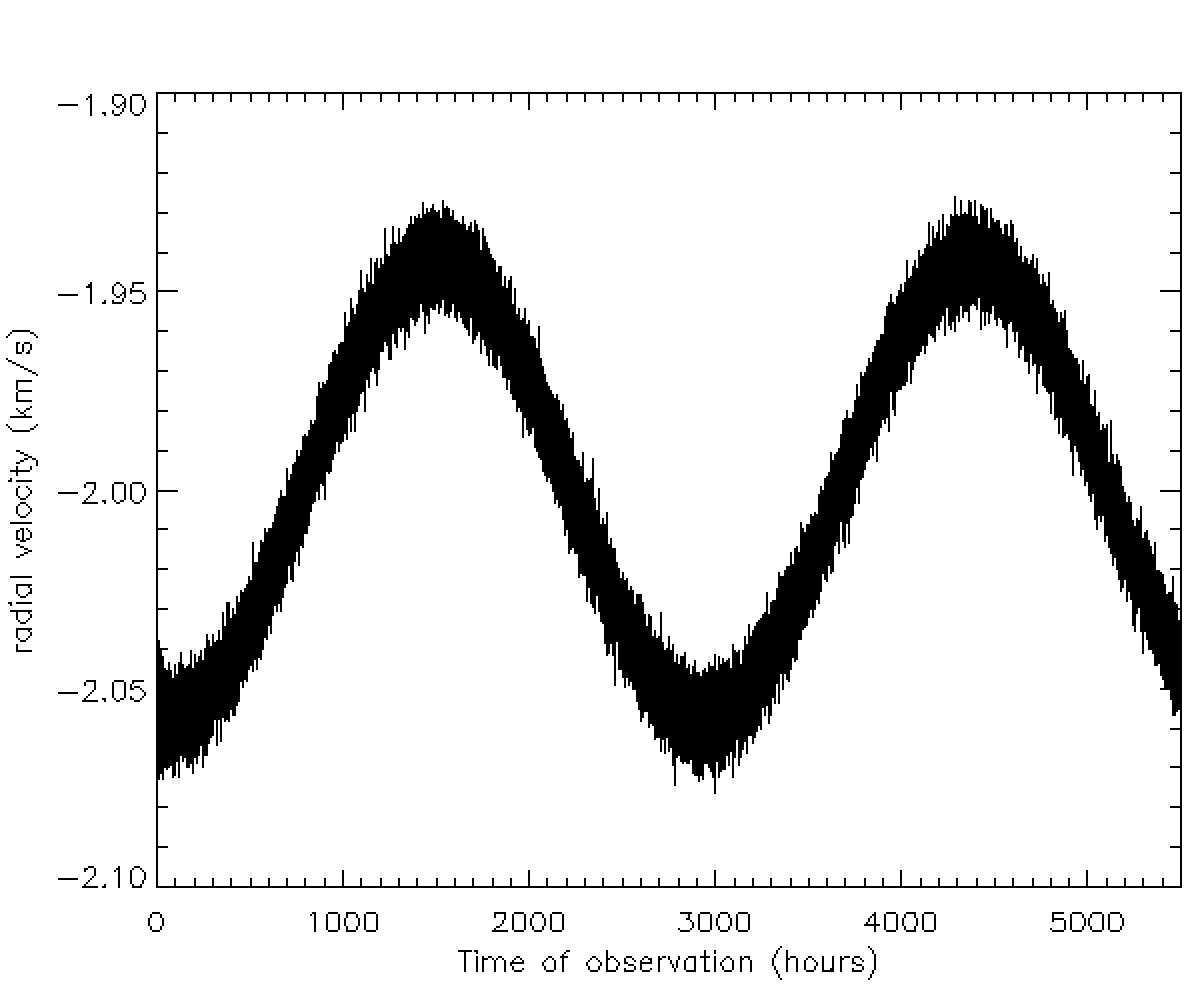
\includegraphics[scale=0.25]{media/vr_nomod.png}\\
\hyperlink{debug2}{\pagebutton{Trykk her!}}
\end{frame}


\begin{frame}
\label{debug2}
\lastpagebutton{debug1}
Du skal altså prøve deg frem med kombinasjoner av verdier for $v_*$, $P$ og $t_0$. Hver kombinasjon gir en modell $v_r^\mathrm{mod}(t_i)$ som du så skal beregne kvadratet av forskjellen til de observerte dataene for. Sånn skal du holde på helt til du finner den kombinasjonen som gir minst mulig forskjell. Hvordan går vi frem? En mulighet er å finne et intervall av mulige parametere for hver av de 3 parameterene. Du kan f.eks. finne den verdien av $t_0$ som passer best ved å se i hvilket intervall denne verdien må ligge. På figuren\\
\centerline{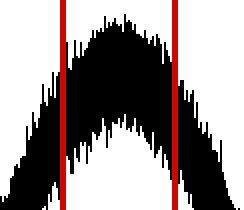
\includegraphics[scale=0.5]{media/vr_t0_int.png}}
ser vi et mulig sånt intervall. Er du enig i at $t_0$ helt sikkert må ligge innenfor dette intervallet? Den kan vel ikke ligge utenfor? (hvis du har glemt hva $t_0$ står for, gå noen sider tilbake, det er viktig at du har dette helt klart for deg!). Del så dette intervallet opp i 20 like steg, og vips du har 20 mulige verdier å prøve for $t_0$. 
\hyperlink{debug3}{\pagebutton{Trykk her!}}
\end{frame}


\begin{frame}
\label{debug3}
\lastpagebutton{debug2}
Vi kan nå gjøre helt det samme for perioden $P$. Er du enig i at perioden (avstanden fra topp til topp) ihvertfall må være større enn avstanden mellom de røde linjene, og ihvertfall mindre enn avstanden mellom de blå linjene. Da har du en minste periode og en største periode som du kan lage f.eks. 20 mulige verdier mellom, akkurat som for $t_0$. Og til slutt gjør du det samme for $v_*$. Da har du til slutt $20^3$ mulige kombinasjoner.\\
\centerline{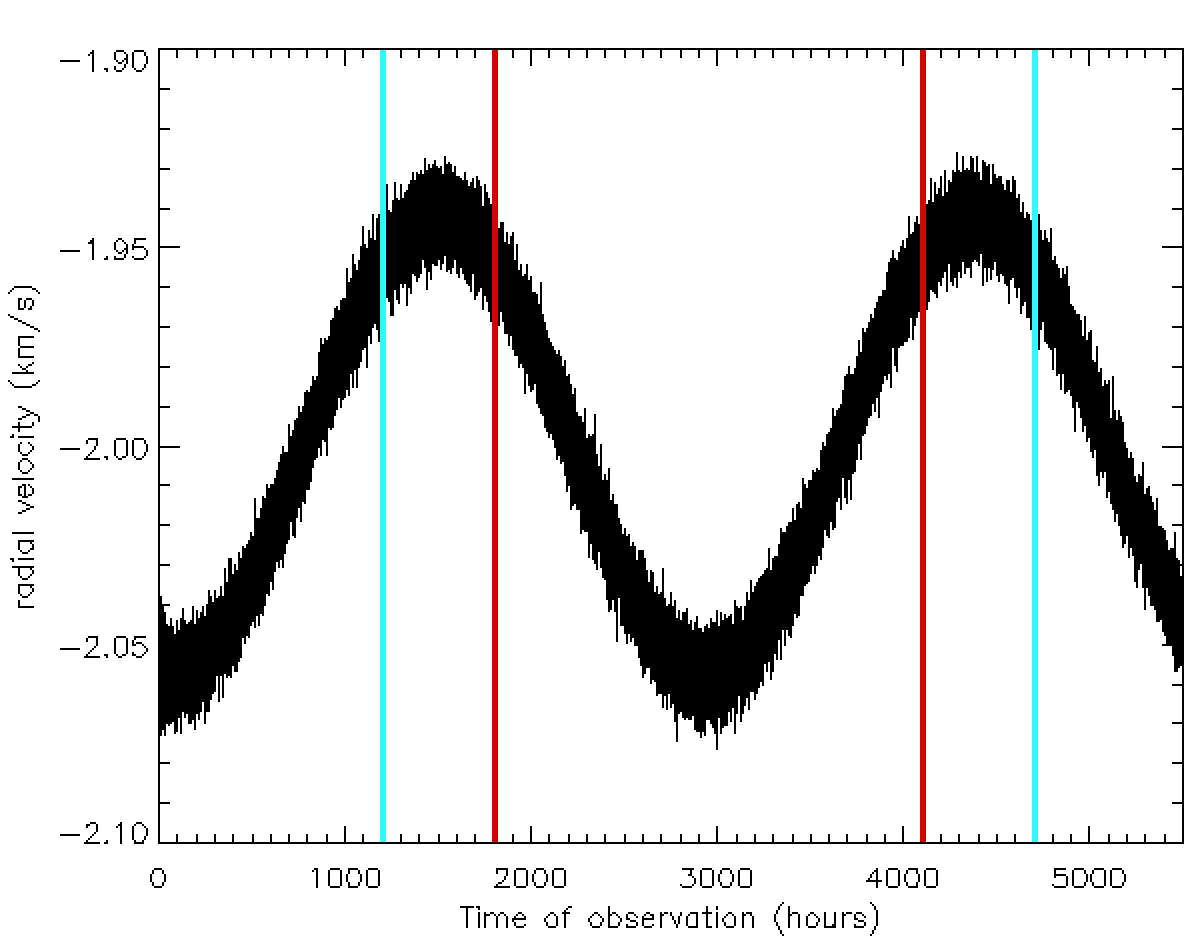
\includegraphics[scale=0.25]{media/vr_p_int.png}}
\hyperlink{debug4}{\pagebutton{Trykk her!}}
\end{frame}




\begin{frame}
\label{debug4}
\lastpagebutton{debug3}
Når du så har funnet den av de $20^3$ kombinasjonene som gir de beste estimatene av $v_*$, $P$ og $t_0$, så kan du tegne modellen $v_r^\mathrm{mod}(t_i)$ og sammenlikne med de observerte dataene. Stemmer det godt overens? Det du spesielt skal tenke på her er om modellen din går midt inne i støyen, husk at støyen er Gaussisk slik at du forventer like mye utslag over som under kurven. Hva gjør du hvis du får et slikt resultat:
\centerline{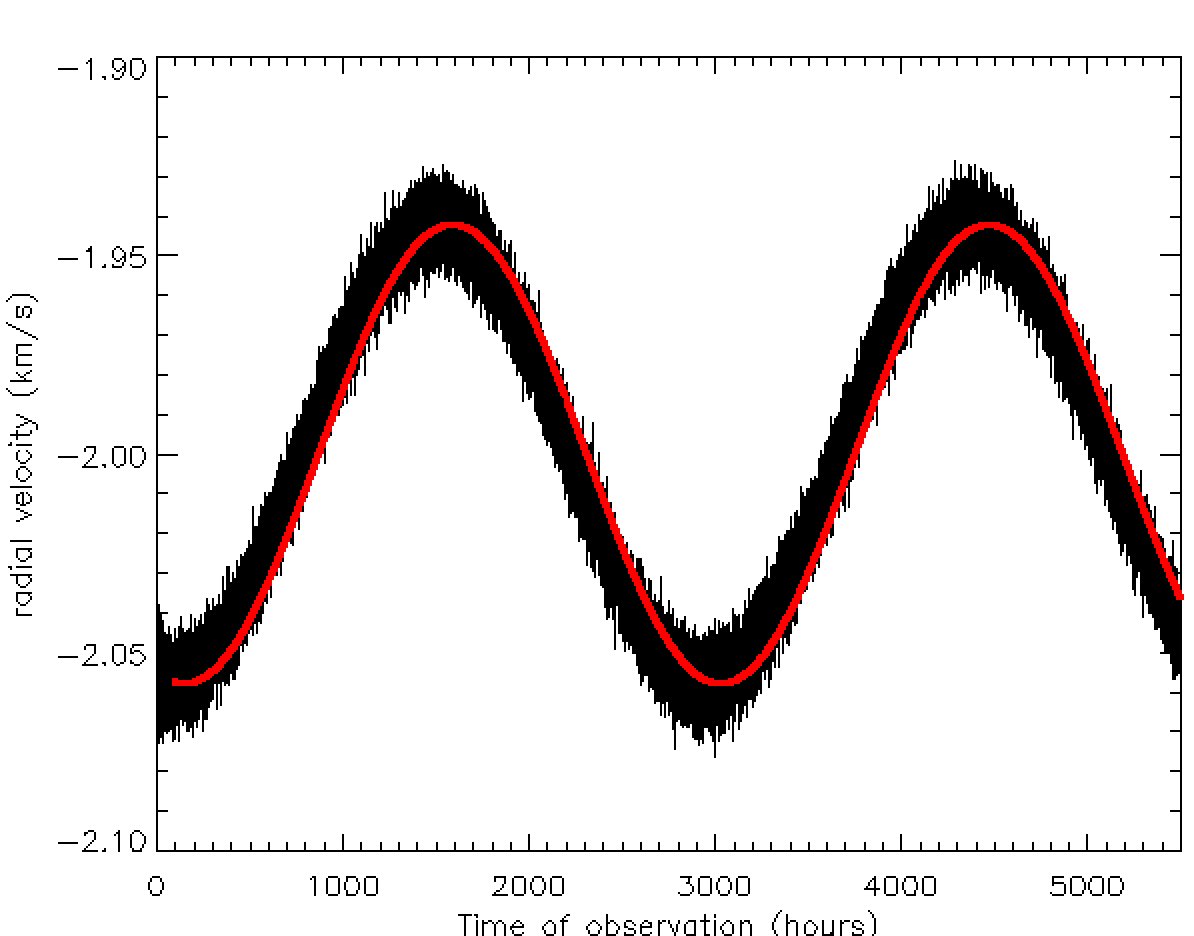
\includegraphics[scale=0.25]{media/vr_wrongmod.png}}
Passer denne modellkurven godt med dataene? Ligger modellkurven midt inne i støyen overalt? Hopper støyen like mye opp som ned overalt på kurven?
\hyperlink{debug4b}{\pagebutton{Trykk her når du har svaret!}}
\end{frame}


\begin{frame}
\label{debug4b}
\lastpagebutton{debug4}
{\Large\bf NEI!} Er du enig i at det {\bf ikke} er tilfelle her? I noen deler av figuren så er støyen nesten hele tiden over eller under modellkurven, den opper ikke like mye over som under!
\centerline{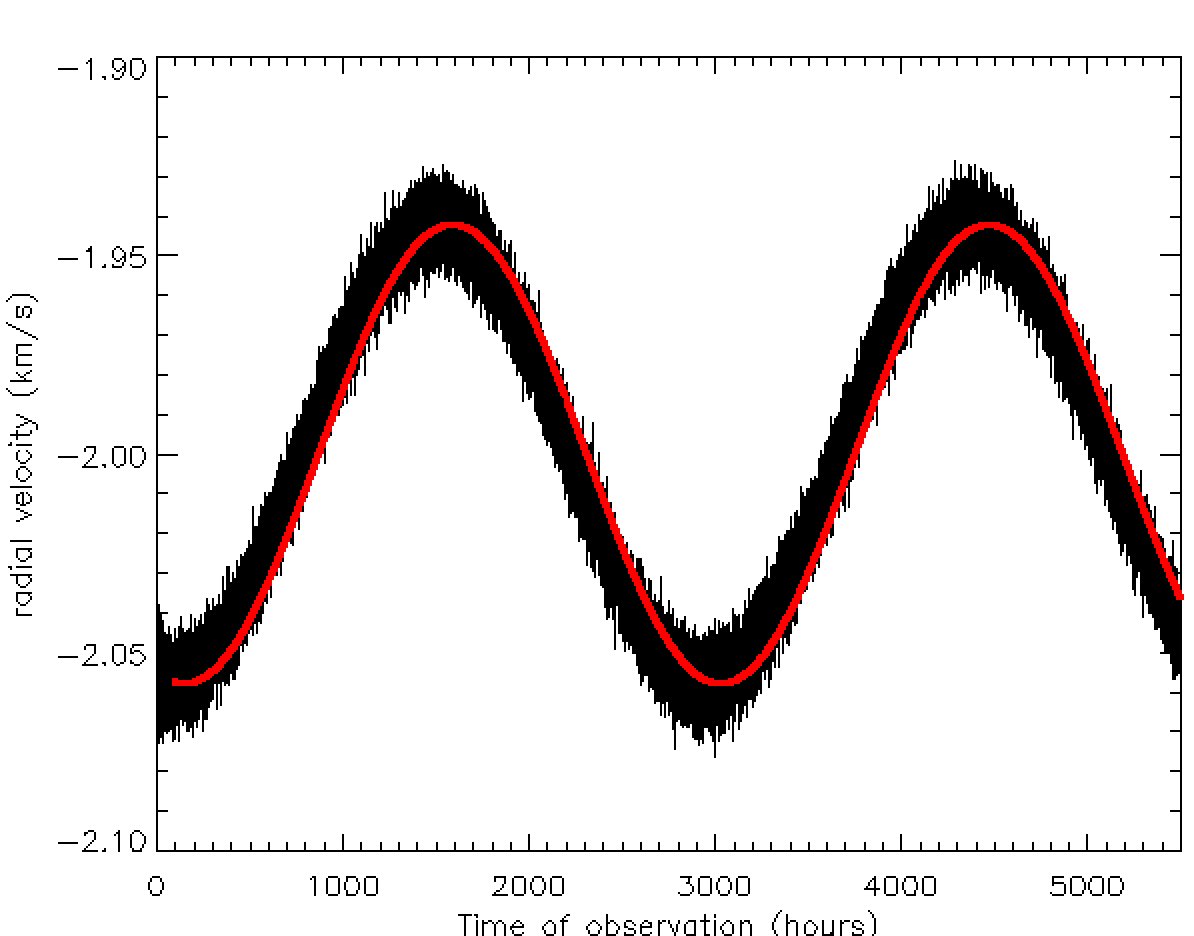
\includegraphics[scale=0.2]{media/vr_wrongmod.png}}
\textcolor{red}{Her kan du være sikker på at noe er feil i koden!}.{\bf Men hvordan skal du finne feilen????}
Her er det selvfølgelig to muligheter:
\begin{itemize}
\item Du har gjort noe feil når du valgte intervallene slik at den beste modellen ikke kommer med!
\item Det er noe feil i koden
\end{itemize}
Aller først bør du dobbeltsjekke at du leste av riktig da du lagde prøve-intervallene for de forskjellige parameterene. Men hvis de er riktige, så må vi debugge...
\hyperlink{debug5}{\pagebutton{Neste side}}
\end{frame}

\begin{frame}
\label{debug5}
\lastpagebutton{debug4b}
\begin{enumerate}
\item Normalt når kurven er så feil at du ser det tydelig slik som her, så er det ganske lett å finne en kurve som passer bedre på øyemål. Gjør så godt du kan for å lese av på figuren og finne en kombinasjon av  $v_*$, $P$ og $t_0$ som du mener passer godt og ihvertfall bedre enn det koden ga deg.
\item Legg til et par linjer i koden som i tillegg til dine $20^3$ kombinasjoner, også tester modellen som du fant ved øyemål. print ut verdien for minste kvadrat (eller $\chi^2$) og sammenlikn med verdien du får for modellen din. Gir modellen din et enda mindre kvadrat?
\item Nå skal du plotte din øyemål-modell over dataene, på samme måte som den røde linjen over. Passer din modell godt? Hvis nei, så ligger sannsynligvis feilen i måten du beregner $v_r^\mathrm{mod}(t_i)$ ifra paramterene $v_*$, $P$ og $t_0$. Hvis du har gjort en god avlesning på øyemål, så {\bf skal} du nå se en kurve som tilsynelatende ser ut til å passe bra. Hvis du har beregnet $v_r^\mathrm{mod}(t_i)$ riktig.
\end{enumerate}
\hyperlink{debug6}{\pagebutton{Neste side}}
\end{frame}


\begin{frame}
\label{debug6}
\lastpagebutton{debug5}
\begin{enumerate}
\setItemnumber{4}
\item Hvis øyemål-modellen din passer ganske bra, ga den en verdi for $\Delta$ eller $\chi^2$ som er mindre enn minste kvadrat-verdien fra de $20^3$ kombinasjonene? Hvis ikke, så er noe galt med måten du beregner  $\Delta$ eller $\chi^2$ på. Husk at disse størrelsene er forskjellen mellom data og modell. Hvis modellen din helt tydelig er bedre, så {\bf må} den også ha en mindre forskjell, enig? Da må du sjekke hvordan du beregner denne forskjellen, hvorfor får du ikke mindre forskjell?
\item Hvis du får mindre forskjell for din modell, så er spørsmålet hvorfor ikke en minst like god modell ble funnet blandt de $20^3$ kombinasjonene. Finn ut hvilken av de $20^3$ kombinasjonene som er nærmest øyemålmodellen din. En enkel måte å gjøre det på er som følger: anta at du hadde 20 prøveverdier for $v_*$, fra $v_*(0)$ som minste prøveverdi og steglengde $\Delta v_*$ slik at største prøveverdi var $v_*(0)+19\times\Delta v_*$. Ta nå din øyemålverdi for $v_*$, del denne på $\Delta v_*$ og rund av til nærmeste heltall. Da har du indeksen blant de 20 prøveverdiene som passer best til din øyemålmodell. 
\end{enumerate}
\hyperlink{debug7}{\pagebutton{Neste side}}
\end{frame}


\begin{frame}
\label{debug7}
\lastpagebutton{debug6}
\begin{enumerate}
\setItemnumber{6}
\item {\bf Pass på: hvis din øyemålmodell er blant de aller første eller alle siste indeksene, altså at den er nær eller under $v_*(0)$, eller nær eller over $v_*(0)+19\times\Delta v_*$, så betyr det at du har valgt intervallet ditt galt slik at den beste løsningen ikke ligger omtrent midt inne i intervallet. Da er feilen rett og slett at du har lest av intervallet galt. Dette er en typisk feil!}
\item Gjør det samme for $P$ og $t_0$. Hvis du fant at alle de 3 verdiene nå ligger omtrent midt i intervallet, \textcolor{red}{så har du funnet den modellen blant de $20^3$ modellene som er nærmest øyemålmodellen din}. Nå skal du gjenta stegene over med denne nye testmodellen. Blir figuren pen med denne modellen også? (det bør den!). Blir  $\Delta$ eller $\chi^2$ mindre enn minste kvadrat fra koden også for denne modellen? (det bør den!). Hvis ja, {\bf hvorfor iallverden ble ikke denne modellen valgt som den beste av de $20^3$ modellene, hvis denne modellen er identisk med en av de $20^3$ modellene?} Da ligger feilen enten i løkken din som gjør at ikke alle  $20^3$ modeller blir loopet gjennom, eller at det er noe galt i selve minimaliseringen.
\end{enumerate}
\hyperlink{oppsummering}{\pagebutton{Neste side}}
\end{frame}

\begin{frame}
\label{oppsummering}
\hyperlink{debug7}{\pagebutton{\small Forrige side}}\href{https://nettskjema.no/a/160191}{\Changey[1][yellow]{2} \Changey[1][yellow]{-2}}
{\Large
Da er vi ferdige med del 1C. Vi har i dette kapittelet sett hvordan vi kan bruke stråling og spektrallinjer til å finne ut om en stjerne har planeter. I del 1D skal vi se nærmere på stråling generelt og spektrallinjer spesielt og den informasjonen som disse kan gi oss om gjerne objekter. I del 1C bør du nå kunne
}
\begin{itemize}
\item Vite hvordan man kan finne ut om en stjerne har en planet i bane rundt seg
\item Forstå sammenhengen mellom en stjernes bane omkring massesenteret til en planet og Dopplereffekten som vi måler fra stjerna.
\item Kunne bruke radialhastighetsgrafer til å anslå massen til planeten
\item Kunne bruke flukskurve ved formørkelse til å anslå planetens radius og tetthet.
\item Forstå hvordan støy påvirker data og hvordan man kan estimere parametere for en teoretisk modell fra data med støy.
\item Forstå hvor minste kvadraters metode og $\chi^2$-metoden kommer fra og kunne bruke disse.
\end{itemize}
\hyperlink{oppsummering2}{\pagebutton{Neste side}}
\end{frame}


\begin{frame}
\label{oppsummering2}
\hyperlink{oppsummering}{\pagebutton{\small Forrige side}}\href{https://nettskjema.no/a/160191}{\Changey[1][yellow]{2} \Changey[1][yellow]{-2}}
{\bf Det anbefales nå at du sjekker \href{https://www.uio.no/studier/emner/matnat/astro/AST2000/h21/undervisningsmateriell/kortsvarsoppgaver/del1c.pdf}{kortsvarsoppgavene} til del 1C for å kontrollere at du har forstått stoffet. Kan du svare på disse, blir det lettere å bruke kunnskapen din i oppgavene/prosjektet. Noen av disse kommer på eksamen.}\\
\vspace*{1cm}  
Trykk nå gjerne på smilefjesene og si meninga di om dette interaktive forelesningsnotatet. Spesielt er jeg interessert i å vite hvor lang tid du brukte og da hva du brukte mest tid på! All ris og ros mottaes med takk for å vite om alt arbeidet med å lage disse interaktive slidene er verd det, om jeg bør fortsette med det og om det er noe jeg bør endre.
\end{frame}

\end{document}
